\PassOptionsToPackage{quiet}{fontspec} %在document{}前加上就可以解决啦!简单暴力!
\documentclass[withoutpreface,bwprint]{cumcmthesis} %去掉封面与编号页
\usepackage{ctex}
\usepackage{multicol}
\usepackage{amsmath}
\usepackage{amssymb}
\usepackage{mathrsfs}
\usepackage{graphics}
\usepackage{subfigure}
\usepackage{float}
\usepackage{booktabs}
\usepackage{color}
\usepackage{xcolor}
\usepackage{listings}
\bibliographystyle{unsrt} %导入的参考文献风格
\usepackage{hyperref}
%改变颜色
\hypersetup{
    colorlinks=true,
    linkcolor=blue,
    filecolor=blue,      
    urlcolor=blue,
    citecolor=cyan,
}

\title{\LaTeX 教学}
\author{陈创禧}

%正文区
\begin{document}
\maketitle

\section*{序言}
Word 的“所见即所得”是一种幻觉。大家都觉得很方便,但是要排版出一篇精美的了论文难度却很大。图片表格经常且不说乱飞,编辑公式的时候,头都大了。有想删除Office的冲动!

\LaTeX 的“所想即所得”是一种现实,它的结构命令便于记忆,格式也可以自动生成,编辑公式一条代码搞定,编号一个环境搞定,爽歪歪!

\LaTeX 的优点实在是太多啦!如果有固定的模板,而且需要写长论文,许多公式,那么\LaTeX 非常好,熟练以后完全不打扰你的写作思路。而且用Latex,长文章,你根本不用担心格式不统一、文件打开慢、做个操作机器会卡住、不同的软件版本样式被改得乱七八糟、公式一多慢得像蜗牛这些问题。我在写重要文章时,就时常担心Word崩溃掉导致内容丢失的问题,还担心哪个地方的行距就莫名其妙不一样了……

一般而言\LaTeX 的缺点是不能所见即所得,需要编译才能看到最终的输出结果。对于长公式而言,初学者往往会非常痛苦。尤其是文章内容多,需要编译的时间很长,公式又很复杂,初学者往往倾向于写一点就要看一下。针对这种问题,你可以新建一个tex文件专门编译正在打的公式。(当然也可像我一样熟练后再长都能一遍过⁄(⁄ ⁄•⁄ω⁄•⁄ ⁄)⁄,其实熟了后看到代码都能直接脑编译的,真的……)

\LaTeX 的学习成本高吗?说低的肯定是骗人的!我也是学习了一天才明白了各种语法,又经过了好几天的练习才慢慢熟练.但是对于我这个学不会Office的人来说\LaTeX 的学习成本相对较低,Office的花样太多了,而且很难排版出一篇满意的了论文和笔记.看到用\LaTeX 排版出来的论文和笔记,很难不爱啊!现在让我回去用Office,我只能说回不去了。

如何高效的使用\LaTeX 的呢?我们可以使用一些\href{https://zhuanlan.zhihu.com/p/516265230}{快捷键}来提高我们的效率。当然啦!还是需要勤加练习。还有要养成良好的使用习惯,一些命令不需要了不要删除,可以使用注释,方便下次使用。刘海洋老师有一句话说得很好,“写作时不排版,排版时不写作。”一心二用办不成好事,我们提前写好内容再进行排版才能大大地提高效率。

如果你受够了 Word 给你带来的「意外」,或许\LaTeX 能给你带来「惊喜」~ 现在就开始\LaTeX 的学习之旅吧!

\begin{multicols}{3}
学习网站:

\begin{itemize}
    \item \href{https://flowus.cn/latex/share/66110e84-b24a-4cd5-b8a7-2ba2afb35a30}{\LaTeX 代码百宝箱}
        \item \href{http://www.uinio.com/Math/LaTex/}{\LaTeX 数学公式语法}

\end{itemize}

书籍:
\begin{itemize}
    \item \href{https://cozier-1315026820.cos.ap-guangzhou.myqcloud.com/epslatex-cn.pdf}{\LaTeX 插图指南}
    \item \href{https://cozier-1315026820.cos.ap-guangzhou.myqcloud.com/%E5%88%98%E6%B5%B7%E6%B4%8B%E3%80%8ALaTeX%E5%85%A5%E9%97%A8%E3%80%8B.pdf}{刘海洋《LaTeX入门》}
\end{itemize}

大牛专刊:
\begin{itemize}
    \item \href{https://www.zhihu.com/people/muzzi/answers}{慕子}
    \item \href{https://www.zhihu.com/people/liu-haiyang}{刘海洋}
\end{itemize}
\end{multicols}

\newpage
\tableofcontents
\newpage
\section{所需软件}
\subsection{\LaTeX}
\begin{enumerate}
    \item 推荐网站: \href{https://texpage.com/}{TeXPage}
    \item 推荐软件: Texlive和TeX studio 
    \href{https://blog.csdn.net/Mikchy/article/details/94448707?ops_request_misc=%257B%2522request%255Fid%2522%253A%2522167843849716800182737093%2522%252C%2522scm%2522%253A%252220140713.130102334..%2522%257D&request_id=167843849716800182737093&biz_id=0&utm_medium=distribute.pc_search_result.none-task-blog-2~all~top_positive~default-1-94448707-null-null.142^v73^insert_down4,201^v4^add_ask,239^v2^insert_chatgpt&utm_term=latex%E5%AE%89%E8%A3%85&spm=1018.2226.3001.4187}{安装教程}
\end{enumerate}

\subsection{公式}
\begin{enumerate}
    \item 推荐网站:
    \begin{itemize}
        \item \href{https://www.latexlive.com/}{在线LaTeX公式编辑器}
        \quad 一个账号每天可以\textbf{免费识别7次}
        \item TexPage内自带识别LaTeX公式的程序可以无限次数使用
    \end{itemize}
    
    \item 推荐软件:\href{https://simpletex.cn/download}{simpletex}
    \par 完全免费!识别质量高,速度也很快,还有很多个性化设置!\textbf{香!实在是太香啦!}
\end{enumerate}

\subsection{图像}
\begin{enumerate}
    \item 建模:MATLAB、Python、Origin、R……
    \item 流程图:
    \begin{itemize}
        \item 软件:PPT、AxGlyph、Visio……
        \item 网站:\href{https://www.processon.com/}{ProcessOn}
    \end{itemize}
\end{enumerate}

\subsection{文献}
\begin{itemize}
    \item \href{https://www.cnki.net/}{中国知网}
    \quad \textbf{可以去某宝买账号,或者使用图书馆的账号}
    \item \href{https://www.oalib.com/}{Open Access Library}
    \item \href{https://ieeexplore.ieee.org/Xplore/home.jsp}{IEEE Xplore}
    \item \href{https://sci-hub.ru/}{Sci-Hub}
    \quad \href{https://zhuanlan.zhihu.com/p/369748238}{IEEE XPLORE论文PDF免费下载方法}
\end{itemize}

\subsection{文献管理}
\begin{enumerate}
    \item 浏览器插件:zotero、jabref
    \item 推荐软件:zotero
    \href{https://www.zotero.org/download/}{下载地址}
\end{enumerate}


\subsection{PDF编辑器}
\begin{itemize}
    \item Adobe Acrobat Reader DC \href{https://pan.baidu.com/s/1YXRn_3ZQIqwByHCHFTIfMA?pwd=v9u7}{破解版下载地址}
    \item 小绿鲸鱼英文文献阅读器
    \href{https://www.xljsci.com/download/index.html}{下载地址}
    \quad \textbf{可以实时翻译文献}
\end{itemize}

\newpage
\section{框架}
\subsection{最基本的结构}
\begin{lstlisting}
%导言区
\documentclass{article}
%\documentclass[withoutpreface,bwprint]{cumcmthesis} %去掉封面与编号页

\usepackage{ctex}

%正文区
\begin{document}
    
\end{document}
\end{lstlisting}

\subsection{源文件的基本结构}
\subsubsection{导言区}
\begin{enumerate}
    \item 文档格式的设置:article, book, report, letter
    \item 文本信息的设置:标题、作者、日期的设置
\end{enumerate}

\begin{lstlisting}
%导言区 
\documentclass{article} %article,book, report, letter 

\title{My First Document} 
\author{Cozier} 
\date{\today} 
\end{lstlisting}

\subsection{正文区}
\begin{enumerate}
    \item 如果有文本信息的设置要加上 \lstinline{\maketitle}
    \item 分段含缩进:\lstinline{\par}或者空格
    \item 分段不含缩进:\lstinline{\\}
    \item 换页:\lstinline{\newpage}
    \item 空格: \lstinline{\quad \qquad \enspace \; \: \, \thinspce \! \negthinspce}
    \item 数学公式:\$\$中间输出的是数学公式,没在里面输出的是文本模式。
    
                    其中一个\$包围的是行内公式,两个\$\$则是行间公式。
    \end{enumerate}

\begin{lstlisting}
%导言区 
\documentclass{article} %article,book, report, letter 

\title{My First Document} 
\author{Cozier} 
\date{\today} 

%正文区(文稿区) \begin{document} 
\maketitle %为了使上面的标题、作者和日期正常显示 

Hello World! 

% $$中间输出的是数学公式,没在里面输出的是文本模式 
% 其中一个$包围的是行内公式,两个$$则是行间公式 

Let $f(x)$ be difined by the formula. 
$f(x)=3x^2+4x+3$. 
$$f(x)=3x^2+4x+3$$ which is a polynomial of degree 2. 

\end{document}
\end{lstlisting}

\section{中文输入及字体}
\subsection{中文输入处理方法}

\subsubsection{法一:调用ctex宏包}
\begin{lstlisting}
\usepackage{ctex}
\end{lstlisting}

\subsubsection{法二:使用ctex文档}
\begin{lstlisting}
\documentclass{ctexart} %ctexbook, ctexrep
\end{lstlisting}

\subsection{中文输入报错警告}
如:Package fontspec Warning: Font "FandolSong-Regulardoes not contain requested Script "CJk".

这些警告不痛不痒,latex还是可以正常编译运行。

让LaTeX 抑制这类警告,假装问题不存在。代码如下:
\begin{lstlisting}
%在document{}前加上就可以解决啦!简单暴力!
\PassOptionsToPackage{quiet}{fontspec} 
\end{lstlisting}

\subsection{字体}
字体设置有两种方法,\textbf{推荐使用字体声明},编辑起来更有结构性,便于修改。

\subsubsection{字体族设置(罗马字体、无衬线字体、打字机字体)}
\begin{lstlisting}
%字体族设置(罗马字体、无衬线字体、打字机字体) 
%第一种是使用字体命令,括号里就是具体内容 
\textrm{Roman Family} \textsf{Sans Serif Family} \texttt{Typewriter Family} 

%第二种是使用字体声明,用于声明后面的字体为罗马字体,大括号用于分组,限定字体限制的范围 
\rmfamily Roman Family {\sffamily Sans Serif Family} {\ttfamily Typewriter Family}
\end{lstlisting}

%字体族设置(罗马字体、无衬线字体、打字机字体) 
%第一种是使用字体命令,括号里就是具体内容 
\textrm{Roman Family} \textsf{Sans Serif Family} \texttt{Typewriter Family} 

%第二种是使用字体声明,用于声明后面的字体为罗马字体,大括号用于分组,限定字体限制的范围 
\rmfamily Roman Family {\sffamily Sans Serif Family} {\ttfamily Typewriter Family}

\subsubsection{字体系列设置(粗细)}
\begin{lstlisting}
%字体系列设置(粗细) 
\textmd{Medium Series} \textbf{Boldface Series}

{\mdseries Medium Series} {\bfseries Boldface Series}
\end{lstlisting}

\textmd{Medium Series} \textbf{Boldface Series}

{\mdseries Medium Series} {\bfseries Boldface Series}

\subsubsection{字体形状设置(直立、斜体、伪斜体、小型大写)}
\begin{lstlisting}
%字体形状设置(直立、斜体、伪斜体、小型大写) 
\textup{Upright Shape} \textit{Italic Shape} \textsl{Slanted Shape} \textsc{Small Caps Shape} 

{\upshape Upright Shape} {\itshape Italic Shape} {\slshape Slanted Shape} {\scshape Small Caps Shape}
\end{lstlisting}

%字体形状设置(直立、斜体、伪斜体、小型大写) 
\textup{Upright Shape} \textit{Italic Shape} \textsl{Slanted Shape} \textsc{Small Caps Shape} 

{\upshape Upright Shape} {\itshape Italic Shape} {\slshape Slanted Shape} {\scshape Small Caps Shape}

\subsubsection{中文字体的设置}
\begin{lstlisting}
%中文字体 
{\songti 宋体} {\heiti 黑体} {\fangsong 仿宋} {\kaishu 楷书} 

%中文字体的粗细和斜体,注意粗体使用黑体表示,斜体使用楷书表示 
\textbf{粗体} \textit{斜体}

{\itshape 斜体} {\bfseries 粗体}
\end{lstlisting}

%中文字体 
{\songti 宋体} {\heiti 黑体} {\fangsong 仿宋} {\kaishu 楷书} 

%中文字体的粗细和斜体,注意粗体使用黑体表示,斜体使用楷书表示 
\textbf{粗体} \textit{斜体}

{\itshape 斜体} {\bfseries 粗体}

\subsubsection{字体大小}
\begin{lstlisting}
%字体大小,都是相对于normal size进行的变化,而normal size在最开始设置,\documentclass[10pt]{article} 
{\tiny Hello}\\ 
{\scriptsize Hello}\\ 
{\footnotesize Hello}\\ 
{\small Hello}\\ 
{\normalsize Hello}\\ 
{\large Hello}\\ 
{\Large Hello}\\ 
{\LARGE Hello}\\ 
{\huge Hello}\\ 
{\Huge Hello}\\ 

%中文字号设置命令 
\zihao{4} 你好!%其中的number 对应Word里的字号大小,负号代表小号,如-4:小四,4:四号
\end{lstlisting}

%字体大小,都是相对于normal size进行的变化,而normal size在最开始设置,\documentclass[10pt]{article} 
{\tiny Hello}\\ 
{\scriptsize Hello}\\ 
{\footnotesize Hello}\\ 
{\small Hello}\\ 
{\normalsize Hello}\\ 
{\large Hello}\\ 
{\Large Hello}\\ 
{\LARGE Hello}\\ 
{\huge Hello}\\ 
{\Huge Hello}\\ 

\section{篇章结构}
\subsection{摘要}
\begin{lstlisting}
%摘要会自动新建页面,并且会根据输入法显示标题[摘要]
\begin{abstract}
内容...

%其中:\quad为两个字符空格
\keywords{内容1 \quad 内容2}
\end{abstract}
\end{lstlisting}

\subsection{提纲建立}
\subsubsection{标题}
\begin{lstlisting}
%一级标题:
\section{内容}

%二级标题:
\subsection{内容}

%三级标题:
\subsubsection{内容}
\end{lstlisting}

\subsubsection{添加目录}
\begin{lstlisting}
\tableofcontent %添加在\section之前,国赛可以不用目录
\end{lstlisting}

\subsection{对原来的设置进行更改}
\subsubsection{设置标题居中}
\begin{lstlisting}
\documentclass{ctexart} %会默认标题居中
\end{lstlisting}

\subsubsection{对section和subsection进行设置}
\begin{lstlisting}
\ctexset{ 
    section ={ 
        format+ = \zihao{-4} \heiti \raggedright, name = {,、}, number = \chinese{section},
        %说明这里的大标题是以中文形式,一、 
        beforeskip = 1.0ex plus 0.2ex minus .2ex, afterskip = 1.0ex plus 0.2ex minus .2ex, aftername = \hspace{0pt}
},
    subsection = { format+ = \zihao{5} \heiti \raggedright, name = {,、}, number = \arabic{section}, beforeskip = 1.0ex plus 0.2ex minus .2ex, afterskip = 1.0ex plus 0.2ex minus .2ex, aftername = \hspace{0pt} 
    } 
}
\end{lstlisting}

\section{列表环境}
\subsection{有序列表}
\begin{lstlisting}
\begin{enumerate}
% \begin{enumerate}[label=(\arabic*)] %带圆括号
% \begin{enumerate}[label=\Roman*] %大写阿拉伯
% \begin{enumerate}[label=\alph*.] %斜体字母
    \item 内容1
    \item 内容2
\end {enumerate}
\end{lstlisting}

\begin{multicols}{4}
\begin{enumerate}
    \item 内容1 
    \item 内容2
\end {enumerate}

\begin{enumerate}[label=(\arabic*)] %带圆括号
    \item 内容1 
    \item 内容2
\end {enumerate}

\begin{enumerate}[label=\Roman*] %大写阿拉伯
    \item 内容1 
    \item 内容2
\end {enumerate}

\begin{enumerate}[label=\alph*.] %斜体字母
    \item 内容1 
    \item 内容2
\end {enumerate}
\end{multicols}

\subsection{无序列表}
\begin{lstlisting}
\begin{itemize}
    \item 内容1
    \item 内容2
\end {itemize}

%无序列表环境--自定义符号:
\begin{itemize}
    \item[-] 内容1 
    \item[+] 内容2
\end{itemize}
\end{lstlisting}

\begin{multicols}{2}
\begin{itemize}
    \item 内容1
    \item 内容2
\end {itemize}

\begin{itemize}
    \item[-] 内容1 
    \item[+] 内容2
\end{itemize}
\end{multicols}

\subsection{解说环境}
\begin{lstlisting}
\begin{description}
    \item[item a] 内容1
    \item[item b] 内容2
\end{description}
\end{lstlisting}

\begin{multicols}{2}
\begin{description}
    \item[item a] 内容1
    \item[item b] 内容2
\end{description}

\end{multicols}

\section{数学公式}

\subsection{特殊符号}
\begin{lstlisting}
\# \$ \% \& \{ \} \_
\^{}           %^输入
\--{}          %-
\textless      %<
\textgreater   %>
\textbar       %|
\textbackslash %\
\end{lstlisting}

\# \$ \% \& \{ \} \_
\^{}           %^输入
\--{}          %-
\textless      %<
\textgreater   %>
\textbar       %|
\textbackslash %\

\subsection{添加宏包}
\begin{lstlisting}
\usepackage{amsmath} 

%输出黑板粗体字符,\mathbb
\usepackage{amssymb}

%输出花体字符,\mathscr
\usepackage{mathrsfs}
\end{lstlisting}

\newpage
\subsection{行内公式}
\begin{enumerate}
    \item single \$ + 公式
    \item 小括号+公式
    \item math的环境
\end{enumerate}

\begin{lstlisting}
美元符号:\par
交换律是
$a+b=b+a$,如$1+2=2+1=3$
\par小括号:\par
交换律是
\(a+b=b+a\),如\(1+2=2+1=3\) 
\par math环境: \par
    交换律是
    \begin{math} 
        a+b=b+a 
    \end{math},如
    \begin{math} 
        1+2=2+1=3 
    \end{math}
\end{lstlisting}

美元符号:\par
交换律是
$a+b=b+a$,如$1+2=2+1=3$

小括号:\par
交换律是
\(a+b=b+a\),如\(1+2=2+1=3\) 

math环境: \par
    交换律是
    \begin{math} 
        a+b=b+a 
    \end{math},如
    \begin{math} 
        1+2=2+1=3 
    \end{math}

\subsection{希腊字母}
小写希腊字母(Lowercase Greek letters )的输入命令为:\lstinline{\alpha,\beta, \gamma}等,相应地,大写形式的输入命令为:\lstinline{\Gamma, \Delta}等。
\quad \href{https://cozier-1315026820.cos.ap-guangzhou.myqcloud.com/symbols.pdf}{完整symbols}

\begin{lstlisting}
$\alpha$\quad $\beta$\quad $\gamma$   %小写
\quad $\Gamma$\quad $\Delta$          %大写
\end{lstlisting}

$\alpha$\quad $\beta$\quad $\gamma$
\quad $\Gamma$\quad $\Delta$

\subsection{上下标} 
\begin{enumerate}
    \item 上标用\^{};下标用\_
    \item 当上下标超过一个字符时,用{}进行分组
\end{enumerate}

\begin{lstlisting}
%上标是通过^符号实现 
$3x^2 - x + 2 = 0$ 

%有时复杂的上边需要用大括号进行分组 
$3x^{20} - x + 2 = 0$ 

$3x^{3y+2} - x + 2 = 0$ 

%下标是通过_下划线来实现 
%分组组要是当上下标超过一个字符就要用大括号 
$a_0,a_1,a_x,a_{xy},a_{100}$
\end{lstlisting}

%上标是通过^符号实现 
$3x^2 - x + 2 = 0$ 

%有时复杂的上边需要用大括号进行分组 
$3x^{20} - x + 2 = 0$ 

$3x^{3y+2} - x + 2 = 0$ 

%下标是通过_下划线来实现 
%分组组要是当上下标超过一个字符就要用大括号 
$a_0,a_1,a_x,a_{xy},a_{100}$

\subsection{分式与根式}
\begin{lstlisting}
%建议都加上{}
%分式
$\frac{1}{2}$\quad $\frac 1 2$\quad $\frac 1 {x+y}$

$\frac{\frac{1}{x}+1}{y+1}$\quad $\frac{\dfrac{1}{x}+1}{y+1}$

%根式
$\sqrt{2}$\quad $\sqrt{x+y}$\quad $\sqrt[3]{2}$
\end{lstlisting}

%建议都加上{}
$\frac{1}{2}$\quad $\frac 1 2$\quad $\frac 1 {x+y}$

$\frac{\frac{1}{x}+1}{y+1}$\quad $\frac{\dfrac{1}{x}+1}{y+1}$

%根式
$\sqrt{2}$\quad $\sqrt{x+y}$\quad $\sqrt[3]{2}$

\subsection{运算符号}
\subsubsection{普通运算符}

函数名通常用罗马字体正体排版,而不是像变量名一样用意大利体排版。
\begin{lstlisting}
%加减乘除
+\quad -\quad $\times$\quad $\cdot$\quad $\div$

%比较运算符
>\quad <\quad $\ge$\quad $\le$\quad $\ne$
\quad $\approx$\quad $\equiv$

%关系运算符
$\cap$\quad $\cup$\quad $\in$\quad $\notin$ \quad
$\subseteq$\quad $\subsetneqq$\quad $\varnothing$

$\forall$\quad $\exists$\quad $\nexists$

$\because$\quad $\therefore$

%数集
$\mathbb{R}$\quad $\mathbb{Q}$\quad $\mathbb{N}$
\quad $\mathbb{N^*}$\quad $\mathbb{Z}$\quad 

%傅里叶变换
$\mathcal{F}$\quad $\mathscr{F}$

%省略号
$\cdots$\quad $\vdots$\quad $\ddots$

%其他
$\infty$\quad $\partial$\quad $\propto$

%三角函数符号
$\sin{x}$\quad $\cos{x}$\quad $\tan{x}$
\quad $\arcsin{x}$\quad $\arccos{x}$\quad $\arctan{x}$
\quad $\sinh{x}$\quad $\cosh{x}$

%对数函数符号
$\log{x}$\quad $\ln{x}$\quad $\log_2{x}$

%极限符号
$\lim\limits_{x \to 0} \frac{x}{\sin{x}}$
\quad $\max{x}$\quad $\min{x}$
\end{lstlisting}

%加减乘除
+\quad -\quad $\times$\quad $\cdot$\quad $\div$

%比较运算符
>\quad <\quad $\ge$\quad $\le$\quad $\ne$
\quad $\approx$\quad $\equiv$

%关系运算符
$\cap$\quad $\cup$\quad $\in$\quad $\notin$ \quad
$\subseteq$\quad $\subsetneqq$\quad $\varnothing$

$\forall$\quad $\exists$\quad $\nexists$

$\because$\quad $\therefore$

%数集
$\mathbb{R}$\quad $\mathbb{Q}$\quad $\mathbb{N}$
\quad $\mathbb{N^*}$\quad $\mathbb{Z}$\quad 

%傅里叶变换
$\mathcal{F}$\quad $\mathscr{F}$

%省略号
$\cdots$\quad $\vdots$\quad $\ddots$

%其他
$\infty$\quad $\partial$\quad $\propto$

%三角函数符号
$\sin{x}$\quad $\cos{x}$\quad $\tan{x}$
\quad $\arcsin{x}$\quad $\arccos{x}$\quad $\arctan{x}$
\quad $\sinh{x}$\quad $\cosh{x}$

%对数函数符号
$\log{x}$\quad $\ln{x}$\quad $\log_2{x}$

%极限符号
$\lim\limits_{x \to 0} \frac{x}{\sin{x}}$
\quad $\max{x}$\quad $\min{x}$

\subsubsection{大型运算符}
\begin{lstlisting}
%求和、求积
$\sum$\quad $\prod$\quad $\sum_i$\quad $\sum_{i=0}^N$
\quad $\frac{\sum_{i=0}^N x_i}{\prod_{i=0}^N x_i}$
\quad $\frac{\sum\limits_{i=0}^N x_i}{\prod\limits_{i=0}^N x_i}$
%积分
$\int$\quad $\iint$\quad $\iiint$\quad $\oint$
\quad $\int_{-\infty}^0 f(x)d{x}$
\quad $\int_{-\infty}^0 f(x) \, \textrm{d{x}}$
\quad $\int\limits_{-\infty}^0 f(x) \, \textrm{d{x}}$
\end{lstlisting}

%求和、求积
$\sum$\quad $\prod$\quad $\sum_i$\quad $\sum_{i=0}^N$
\quad $\frac{\sum_{i=0}^N x_i}{\prod_{i=0}^N x_i}$\quad $\frac{\sum\limits_{i=0}^N x_i}{\prod\limits_{i=0}^N x_i}$

%积分
$\int$\quad $\iint$\quad $\iiint$\quad $\oint$
\quad $\int_{-\infty}^0 f(x)d{x}$
\quad $\int_{-\infty}^0 f(x) \, \textrm{d{x}}$
\quad $\int\limits_{-\infty}^0 f(x) \, \textrm{d{x}}$

\subsection{标注符号}
\begin{lstlisting}
%向量
$\Vec{x}$\quad $\overrightarrow{AB}$

%平均值
$\Bar{x}$\quad $\overline{AB}$
\end{lstlisting}

%向量
$\Vec{x}$\quad $\overrightarrow{AB}$

%平均值
$\Bar{x}$\quad $\overline{AB}$

\subsection{箭头}
\begin{lstlisting}
%短箭头
$\leftarrow$\quad $\rightarrow$\quad $\Leftarrow$
\quad $\Rightarrow$\quad $\Leftrightarrow$

%长单箭头
$\longleftarrow$\quad $\longrightarrow$\quad $\longleftarrow$\quad $\longrightarrow$\quad $\longleftrightarrow$

%长双箭头
$\Longleftarrow$\quad $\Longrightarrow$\quad $\Longleftarrow$\quad $\Longrightarrow$\quad $\Longleftrightarrow$
\end{lstlisting}

%短箭头
$\leftarrow$\quad $\rightarrow$\quad $\Leftarrow$
\quad $\Rightarrow$\quad $\Leftrightarrow$

%长单箭头
$\longleftarrow$\quad $\longrightarrow$\quad $\longleftarrow$\quad $\longrightarrow$\quad $\longleftrightarrow$

%长双箭头
$\Longleftarrow$\quad $\Longrightarrow$\quad $\Longleftarrow$\quad $\Longrightarrow$\quad $\Longleftrightarrow$

\subsection{括号与定界符}
\begin{lstlisting}
%括号
()\quad []\quad \{\}

%定界符
$(0,\frac{1}{a}]$\quad $\left(0,\frac{1}{a}\right]$\par
$\frac{1}{t}\sqrt{1+t^{2}}|_1 ^{\frac{1}{2}}$
\quad $\left.\dfrac{1}{t}\sqrt{1+t^{2}}\right|_1 ^{\frac{1}{2}}$ %虚空括号
\end{lstlisting}

%括号
()\quad []\quad \{\}

%定界符
$(0,\frac{1}{a}]$\quad $\left(0,\frac{1}{a}\right]$\par
$\frac{1}{t}\sqrt{1+t^{2}}|_1 ^{\frac{1}{2}}$
\quad $\left.\dfrac{1}{t}\sqrt{1+t^{2}}\right|_1 ^{\frac{1}{2}}$ %虚空括号

\subsection{多行数学公式}
\subsubsection{gather环境}
\begin{lstlisting}
   %gather环境,不仅实现多行公式的排版,而且可以自动编号
    \begin{gather}
        a + b  =b + a \\
        a\times b = b\times a
    \end{gather}
    %gather*环境,不带编号的多行公式排版
    \begin{gather*}
        a + b = b + a \\
        a\times b = b\times a
    \end{gather*}
    %也可以在某一行换行之前使用\notag命令,取消这一行公示的编号
    \begin{gather}
        a + b = b + a \\
        a\times b = b\times a \notag \\
        2 \times 3 = 3 \times 2 = 6
    \end{gather}
\end{lstlisting}
   %gather环境,不仅实现多行公式的排版,而且可以自动编号
    \begin{gather}
        a + b  =b + a \\
        a\times b = b\times a
    \end{gather}
    %gather*环境,不带编号的多行公式排版
    \begin{gather*}
        a + b = b + a \\
        a\times b = b\times a
    \end{gather*}
    %也可以在某一行换行之前使用\notag命令,取消这一行公示的编号
    \begin{gather}
        a + b = b + a \\
        a\times b = b\times a \notag \\
        2 \times 3 = 3 \times 2 = 6
    \end{gather}

\subsubsection{align环境}
\begin{lstlisting}
%实现公式之间的对齐,可以使用align和align*(用&指定对齐位置)
    %带编号 
    \begin{align} 
        x &= t + \cos t +1 \\ 
        y &= 2\sin t 
    \end{align} 
    
    %不代编号以及多个公式分别对齐 
    %如等号对齐,每个开头对齐 
    \begin{align*} 
        x &= t & x &= \cos t & x &=t \\ 
        y &=2t & y &= \sin (t+1) & y &= \sin t 
    \end{align*}
\end{lstlisting}
    %实现公式之间的对齐,可以使用align和align*(用&指定对齐位置)
    %带编号 
    \begin{align} 
        x &= t + \cos t +1 \\ 
        y &= 2\sin t 
    \end{align} 
    %不代编号以及多个公式分别对齐 
    %如等号对齐,每个开头对齐 
    \begin{align*} 
        x &= t & x &= \cos t & x &=t \\ 
        y &=2t & y &= \sin (t+1) & y &= \sin t 
    \end{align*}

\newpage
\subsubsection{split环境}
\begin{lstlisting}
    %split环境(对齐采用align环境的方式,编号在中间,主要适用于连等符号,也就是一个公式多行排版) 
    %在equation环境下 
    \begin{equation} 
        \begin{split} 
            \cos 2x &= \cos^2 x - \sin^2 x \\ 
            &= 2\cos^2 x - 1 
        \end{split} 
    \end{equation}
\end{lstlisting}
    %split环境(对齐采用align环境的方式,编号在中间,主要适用于连等符号,也就是一个公式多行排版) 
    %在equation环境下 
    \begin{equation} 
        \begin{split} 
            \cos 2x &= \cos^2 x - \sin^2 x \\ 
            &= 2\cos^2 x - 1 
        \end{split} 
    \end{equation}

\subsubsection{cases环境}
\begin{lstlisting}
 %cases 环境,用于分段函数的表示 
    %每行公式中使用&分隔符为连各个部分 
    %通常表示值和后面的条件 
    %在equation环境下 
    %\in表示的是属于符号,\textem{}表示在公式环境下输出文本 
    \begin{equation} 
        D(x) = \begin{cases} 
            1, & \textrm{如果 } x \in \mathbb{Q} \\ 
            0, & \textrm{如果 } x \in \mathbb{R} \setminus\mathbb{Q}. 
        \end{cases} 
    \end{equation}
\end{lstlisting}
    %cases 环境,用于分段函数的表示 
    %每行公式中使用&分隔符为连各个部分 
    %通常表示值和后面的条件 
    %在equation环境下 
    %\in表示的是属于符号,\textem{}表示在公式环境下输出文本 
    \begin{equation} 
        D(x) = \begin{cases} 
            1, & \textrm{如果 } x \in \mathbb{Q} \\ 
            0, & \textrm{如果 } x \in \mathbb{R} \setminus\mathbb{Q}. 
        \end{cases} 
    \end{equation}

\subsection{实战演练}

\[ 
\sigma=\sqrt{\dfrac{\sum(x_i-\overline{x})^2}{n-1}}\quad(n\to\infty)
\]

\[ 
\lim\limits_{n\to\infty}P\left\{\left|\dfrac{I\left(\alpha_i\right)}{N}-H(s) \right|<\varepsilon\right\}=1
\]

\[ 
x(n)=\dfrac{1}{2\pi} \int_{-\pi}^{\pi} X \left(\mathrm{e}^{\mathrm{j}\omega} \right)\mathrm{e}^{\mathrm{j}\omega n}\,\mathrm{d}\omega
\]

\begin{lstlisting}
	\[ 
	\sigma=\sqrt{\dfrac{\sum(x_i-\overline{x})^2}{n-1}}\quad(n\to\infty)
	\]
	
	\[ 
	\lim\limits_{n\to\infty}P\left\{\left|\dfrac{I\left(\alpha_i\right)}{N}-H(s) \right|<\varepsilon\right\}=1
	\]
	
	\[ 
	x(n)=\dfrac{1}{2\pi} \int_{-\pi}^{\pi} X \left(\mathrm{e}^{\mathrm{j}\omega} \right)\mathrm{e}^{\mathrm{j}\omega n}\,\mathrm{d}\omega
	\]
\end{lstlisting}
\newpage
\section{矩阵}
\subsection{常见矩阵环境}
\begin{lstlisting}
\begin{multicols}{3}
%无括号环境
\(\begin{matrix}

    a & b & \cdots & c \\
    \vdots& \vdots & \ddots &\vdots \\
    e & f & \cdots & g \\

\end{matrix}\)

%圆括号环境
\(\begin{pmatrix}

    a & b & \cdots & c \\
    \vdots& \vdots & \ddots &\vdots \\
    e & f & \cdots & g \\

\end{pmatrix}\)

%方括号环境
\(\begin{bmatrix}

    a & b & \cdots & c \\
    \vdots& \vdots & \ddots &\vdots \\
    e & f & \cdots & g \\

\end{bmatrix}\)
\end{multicols}

\begin{multicols}{3}
%单竖线环境
\(\begin{vmatrix}

    a & b & \cdots & c \\
    \vdots& \vdots & \ddots &\vdots \\
    e & f & \cdots & g \\

\end{vmatrix}\)

%大括号环境
\(\begin{Bmatrix}

    a & b & \cdots & c \\
    \vdots& \vdots & \ddots &\vdots \\
    e & f & \cdots & g \\

\end{Bmatrix}\)

%双竖线环境
\(\begin{Vmatrix}

    a & b & \cdots & c \\
    \vdots& \vdots & \ddots &\vdots \\
    e & f & \cdots & g \\

\end{Vmatrix}\)
\end{multicols}
\end{lstlisting}

\begin{multicols}{3}
%无括号环境
\(\begin{matrix}

    a & b & \cdots & c \\
    \vdots& \vdots & \ddots &\vdots \\
    e & f & \cdots & g \\

\end{matrix}\)

%圆括号环境
\(\begin{pmatrix}

    a & b & \cdots & c \\
    \vdots& \vdots & \ddots &\vdots \\
    e & f & \cdots & g \\

\end{pmatrix}\)

%方括号环境
\(\begin{bmatrix}

    a & b & \cdots & c \\
    \vdots& \vdots & \ddots &\vdots \\
    e & f & \cdots & g \\

\end{bmatrix}\)
\end{multicols}

\begin{multicols}{3}
%单竖线环境
\(\begin{vmatrix}

    a & b & \cdots & c \\
    \vdots& \vdots & \ddots &\vdots \\
    e & f & \cdots & g \\

\end{vmatrix}\)

%大括号环境
\(\begin{Bmatrix}

    a & b & \cdots & c \\
    \vdots& \vdots & \ddots &\vdots \\
    e & f & \cdots & g \\

\end{Bmatrix}\)

%双竖线环境
\(\begin{Vmatrix}

    a & b & \cdots & c \\
    \vdots& \vdots & \ddots &\vdots \\
    e & f & \cdots & g \\

\end{Vmatrix}\)
\end{multicols}

\newpage
\subsection{规范的矩阵写法}
矩阵要用加粗的罗马体写,转置也需要用罗马写。

在数学公式里,加粗的命令和直立体的命令与文本是不同的。
\begin{lstlisting}
\mathbf{}    %加粗罗马体
\mathrm{}    %罗马体
\end{lstlisting}

\begin{lstlisting}
\begin{multicols}{2}
\[
\mathbf{A}=\begin{bmatrix}

    a & b & \cdots & c \\
    \vdots& \vdots & \ddots &\vdots \\
    e & f & \cdots & g \\

\end{bmatrix}
\]

\[
\mathbf{B}^{\mathrm{T}}=\begin{bmatrix}

    a & b & \cdots & c \\
    \vdots& \vdots & \ddots &\vdots \\
    e & f & \cdots & g \\

\end{bmatrix}
\]
\end{multicols}
\end{lstlisting}

\begin{multicols}{2}
\[
\mathbf{A}=\begin{bmatrix}

    a & b & \cdots & c \\
    \vdots& \vdots & \ddots &\vdots \\
    e & f & \cdots & g \\

\end{bmatrix}
\]

\[
\mathbf{B}^{\mathrm{T}}=\begin{bmatrix}

    a & b & \cdots & c \\
    \vdots& \vdots & \ddots &\vdots \\
    e & f & \cdots & g \\

\end{bmatrix}
\]
\end{multicols}

\newpage
\subsection{三角矩阵}
\begin{lstlisting}
%三角矩阵 
%\multicolumn{cols}{pos}{text}合并多列 
%\raisebox调整高度 
\[ 
\begin{pmatrix} 
a_{11} & a_{12} & \cdots & a_{1n} \\
& a_{22} & \cdots & a_{2n} \\ 
& & \ddots & \vdots \\ 
\multicolumn{2}{c}{\raisebox{1.3ex}[0pt]{\Huge 0}}& &a_{nn} 
\end{pmatrix} 
\]
\end{lstlisting}

%三角矩阵 
%\multicolumn{cols}{pos}{text}合并多列 
%\raisebox调整高度 
\[ 
\begin{pmatrix} 
a_{11} & a_{12} & \cdots & a_{1n} \\
& a_{22} & \cdots & a_{2n} \\ 
& & \ddots & \vdots \\ 
\multicolumn{2}{c}{\raisebox{1.3ex}[0pt]{\Huge 0}}& &a_{nn} 
\end{pmatrix} 
\]

\subsection{分块矩阵}

\subsubsection{不含虚实线}
\begin{lstlisting}
%分块矩阵(矩阵嵌套) 
%在数学公式中\Large 0和\textrm{\Large 0}表示的不一样 
 \[ 
 \begin{pmatrix} 
     \begin{matrix} 
         1&0 \\ 0&1 
     \end{matrix} & \mathbf{\Large O} \\ 
     \mathbf{\Large O} & \begin{matrix} 
         1&0 \\ 0&1 
     \end{matrix} 
 \end{pmatrix} 
 \]
\end{lstlisting}

%分块矩阵(矩阵嵌套) 
%在数学公式中\Large 0和\textrm{\Large 0}表示的不一样 
 \[ 
 \begin{pmatrix} 
     \begin{matrix} 
         1&0 \\ 0&1 
     \end{matrix} & \mathbf{\Large O} \\ 
     \mathbf{\Large O} & \begin{matrix} 
         1&0 \\ 0&1 
     \end{matrix} 
 \end{pmatrix} 
 \]

\subsubsection{含横竖实线}
\begin{lstlisting}
\begin{multicols}{3}
\[
\left[\begin{array}{cc|cc}
    a & b & c & d\\
    a & b & c & d\\
    a & b & c & d\\ 
    a & b & c & d\\ 
\end{array}\right]
\]
\[
\left[\begin{array}{cccc}
    a & b & c & d\\
    a & b & c & d\\
    \hline
    a & b & c & d\\ 
    a & b & c & d\\ 
\end{array}\right]
\]
\[
\left[\begin{array}{cc|cc}
    a & b & c & d\\
    a & b & c & d\\
    \hline
    a & b & c & d\\ 
    a & b & c & d\\ 
\end{array}\right]
\]
\end{multicols}
\end{lstlisting}

\begin{multicols}{3}
\[
\left[\begin{array}{cc|cc}
    a & b & c & d\\
    a & b & c & d\\
    a & b & c & d\\ 
    a & b & c & d\\ 
\end{array}\right]
\]

\[
\left[\begin{array}{cccc}
    a & b & c & d\\
    a & b & c & d\\
    \hline
    a & b & c & d\\ 
    a & b & c & d\\ 
\end{array}\right]
\]

\[
\left[\begin{array}{cc|cc}
    a & b & c & d\\
    a & b & c & d\\
    \hline
    a & b & c & d\\ 
    a & b & c & d\\ 
\end{array}\right]
\]
\end{multicols}

\subsection{行内小矩阵}
\begin{lstlisting}
%smallmatrix环境
复数 $z = (x,y)$ 也可以用矩阵 
\begin{math} 
    \left(%需要手动加上左括号 
        \begin{smallmatrix} 
            x & -y \\ y & x 
        \end{smallmatrix} 
        \right)%需要手动加上右括号 
    \end{math}来表示。
\end{lstlisting}

%smallmatrix环境
复数 $z = (x,y)$ 也可以用矩阵 
\begin{math} 
    \left(%需要手动加上左括号 
        \begin{smallmatrix} 
            x & -y \\ y & x 
        \end{smallmatrix} 
        \right)%需要手动加上右括号 
    \end{math}来表示。

\subsection{array环境}
\begin{lstlisting}
%array环境(类似于表格环境tabular) 
%引入array矩阵可以插入更为复杂的矩阵 
\[ 
\begin{array}{r|r} 
    \frac 12 & 0 \\ 
    \hline 0 & -\frac a{bc} \\ 
\end{array} 
\]
\end{lstlisting}

%array环境(类似于表格环境tabular) 
%引入array矩阵可以插入更为复杂的矩阵 
\[ 
\begin{array}{r|r} 
    \frac 12 & 0 \\ 
    \hline 0 & -\frac a{bc} \\ 
\end{array} 
\]

\section{插图}
\subsection{浮动体}
\begin{enumerate}
    \item h此处(here)浮动体的内容被放在代码所在的上下文位置。
    \item t顶端(top):表示优先将图片放置在页面对应排的顶部。
    \item b底端(bottom):表示优先将图片放置在页面对应排的底部。
    \item p浮动页(float page):浮动页。此类浮动体会尝试单独成页。
\end{enumerate}

\subsection{使用浮动体的建议}
\begin{itemize}
    \item 首先要知道如何引用图片【养成在所属文件夹建立图片文件夹的习惯】
    \item 其次如何知道对图片大小和样式进行设置
    \item 对图片或者表格的排版、命名、标签和交叉使用
    \item 在大的figure、table的标签下面去写小的图片或者表格
\end{itemize}

\subsection{限制浮动效果}

有时候图片会乱跑,我们可以强行限制浮动体。就像乱跑的小朋友要打一顿才会乖乖地待在原地。
\begin{lstlisting} 
%导入宏包
\usepackage{float}  

%使用方式
\begin{figure}[H]
图片
\end{figure}
\end{lstlisting}

\subsection{1×1类型(共享标题)}
\subsubsection{添加宏包}
\begin{lstlisting}
%引用图片宏包
\usepackage{graphicx}

%用于排版图片位置
\usepackage{float}	
\end{lstlisting}

\subsubsection{模板}
\begin{lstlisting}
\begin{figure}[H]%开始引用图片环境,[H]为固定图片,防止图片乱跑
    \centering%使图片居中
    %插入图片的命令,[scale]为图片大小,后面跟着图片的路径和名字。也可以使用width和height更改图片的大小
    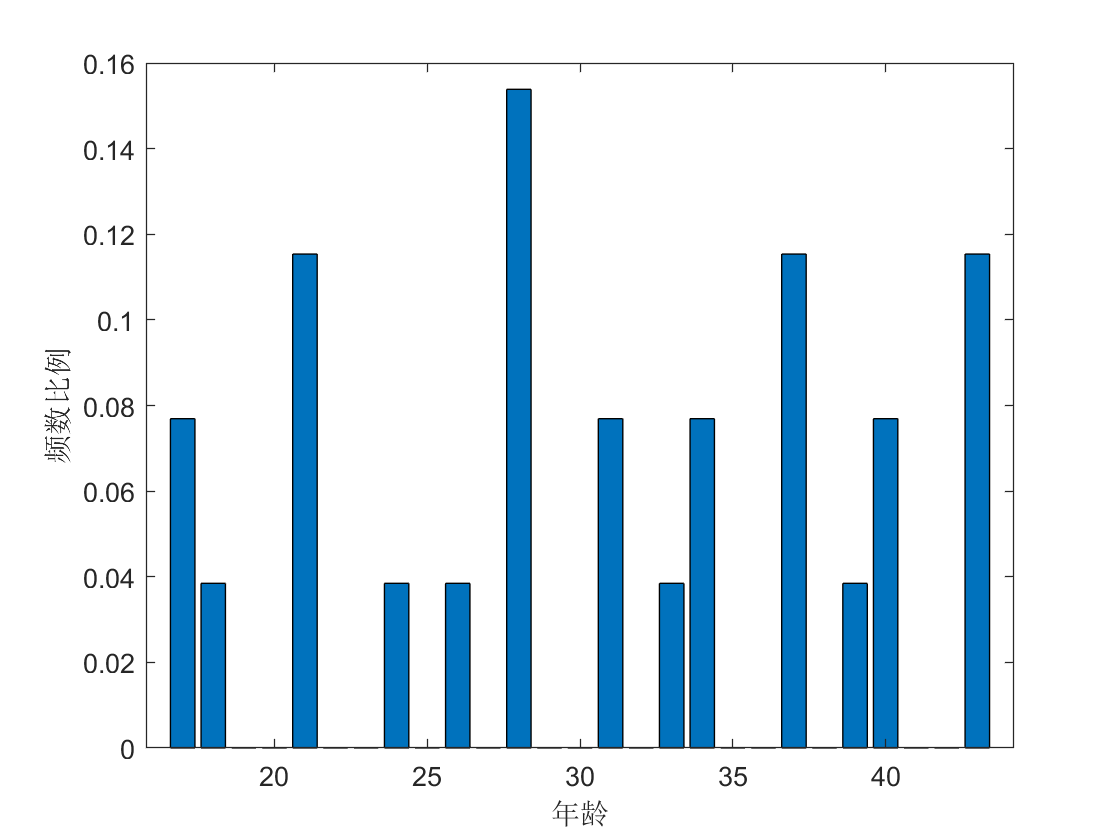
\includegraphics[scale=0.4]{figure/1.png}
    \caption{柱状图}%显示图名
    \label{柱状图}%给图片定义一个标签,用于引用
\end{figure}%结束引用图片环境
这个就是导入的单张图片图片,如图\ref{柱状图}:
\end{lstlisting}

\begin{figure}[H]%开始引用图片环境,[H]为固定图片,防止图片乱跑
    \centering%使图片居中
    %插入图片的命令,[scale]为图片大小,后面跟着图片的路径和名字,可以使用width和height更改图片的大小
    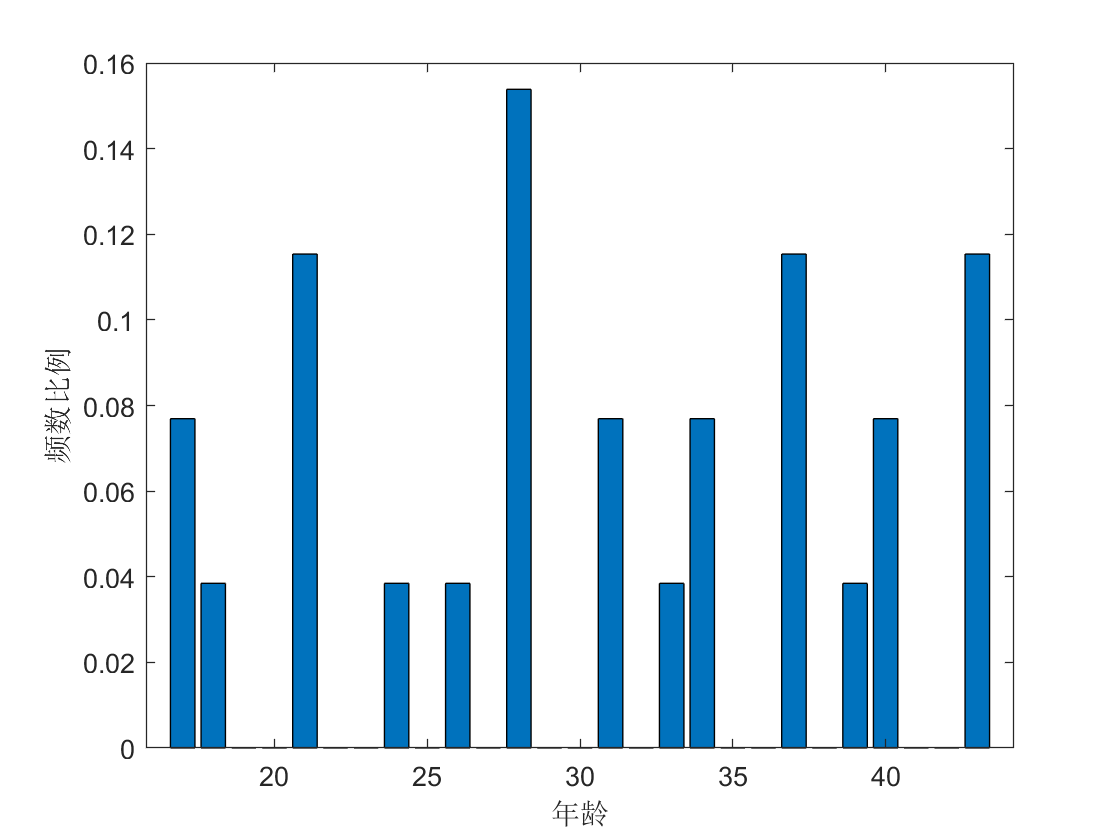
\includegraphics[scale=0.5]{figure/1.png}
    \caption{柱状图}%显示图名
    \label{柱状图}%给图片定义一个标签,用于引用
\end{figure}%结束引用图片环境
这个就是导入的单张图片图片,如图\ref{柱状图}:

\newpage
\subsection{2×2类型(独立标题)}
\begin{lstlisting}
\begin{figure}[H]
    \centering
        \subfigure[标题一]
        {
        \begin{minipage}[b]{0.45\textwidth}
        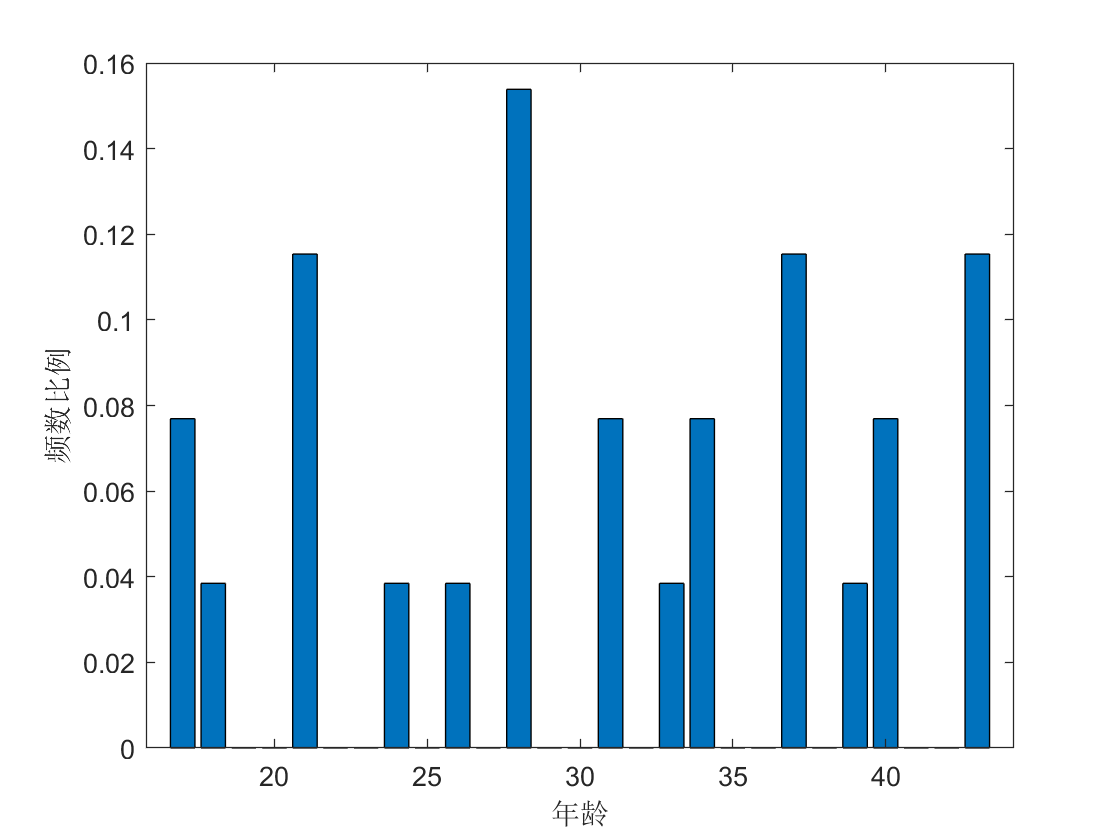
\includegraphics[width=1\textwidth]{figure/1.png}
        \end{minipage}
            \label{fig:1}
        }
        \subfigure[标题二]
        {
        \begin{minipage}[b]{0.45\textwidth}
        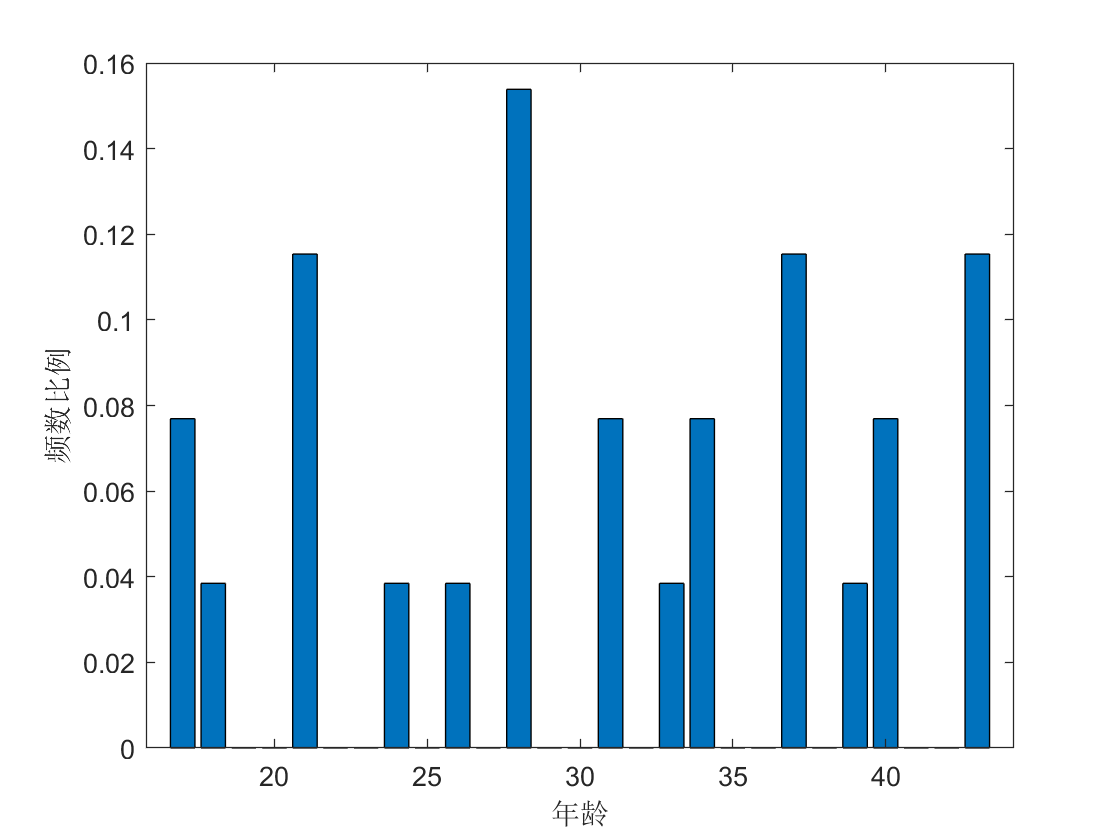
\includegraphics[width=1\textwidth]{figure/1.png}
        \end{minipage}
            \label{fig:2}
        } \\
        \subfigure[标题三]
        {
        \begin{minipage}[b]{0.45\textwidth}
        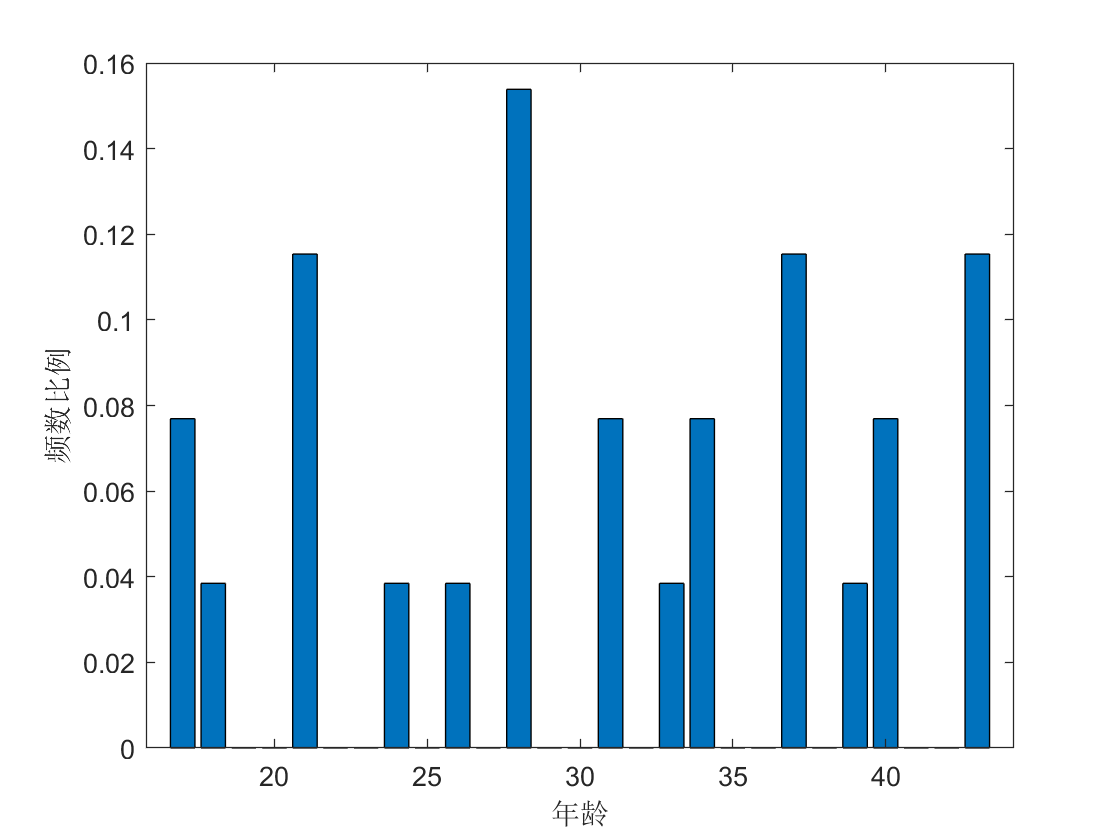
\includegraphics[width=1\textwidth]{figure/1.png}
        \end{minipage}
            \label{fig:3}
        }
        \subfigure[标题四]
        {
        \begin{minipage}[b]{0.45\textwidth}
        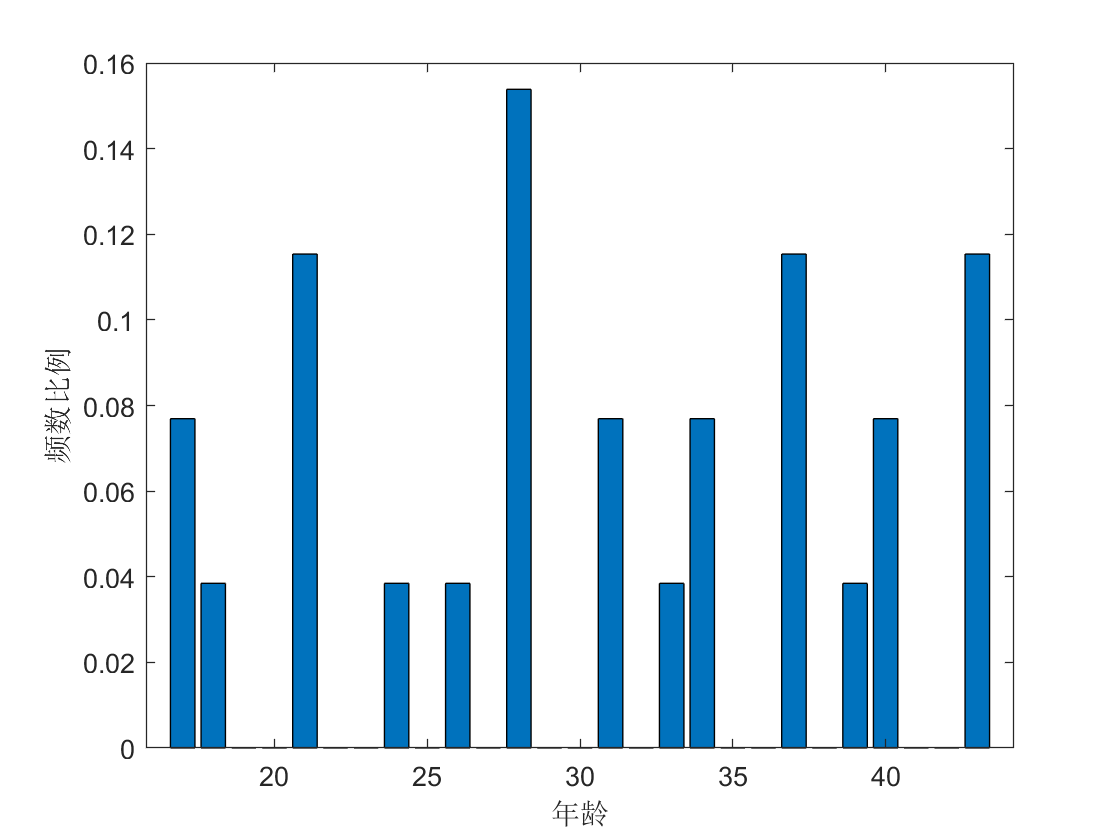
\includegraphics[width=1\textwidth]{figure/1.png}
        \end{minipage}
            \label{fig:4}
        }
        \caption{四图栅格布局摆放,统一大标题,独立子标题}
            \label{fig:5}
\end{figure}
\end{lstlisting}

\begin{figure}[H]
    \centering
        \subfigure[标题一]
        {
        \begin{minipage}[b]{0.45\textwidth}
        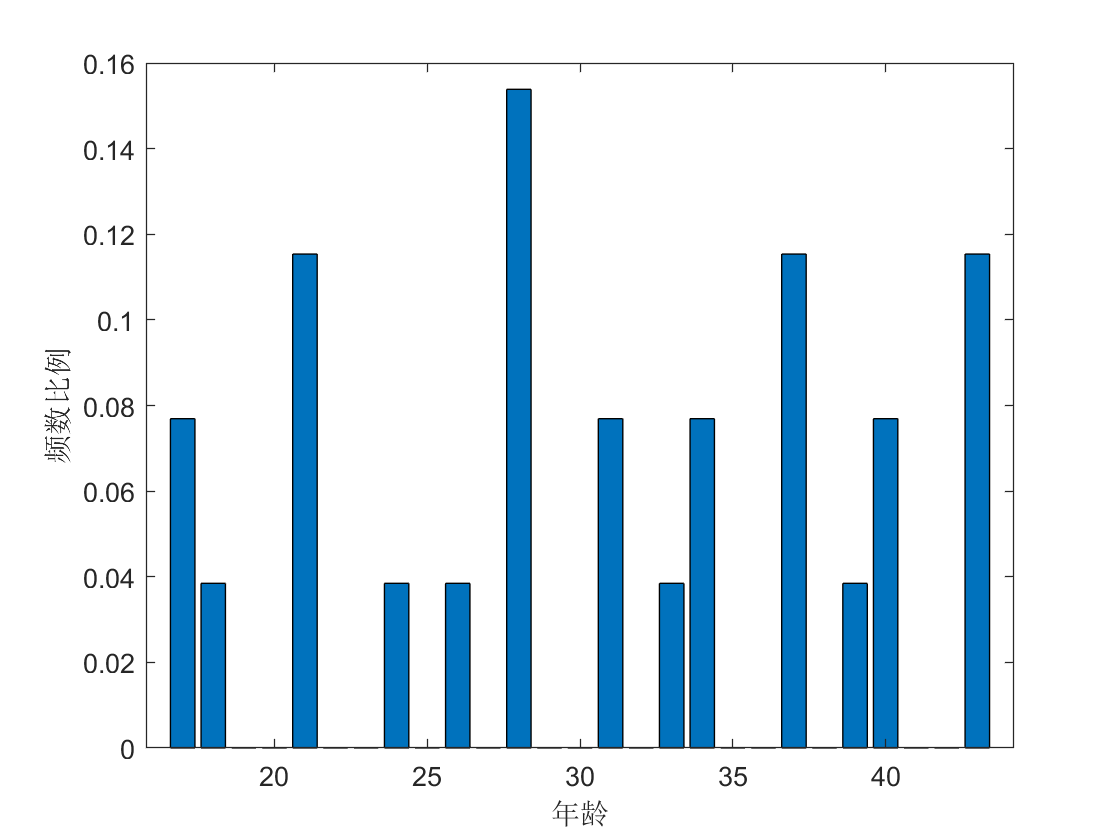
\includegraphics[width=1\textwidth]{figure/1.png}
        \end{minipage}
            \label{fig:1}
        }
        \subfigure[标题二]
        {
        \begin{minipage}[b]{0.45\textwidth}
        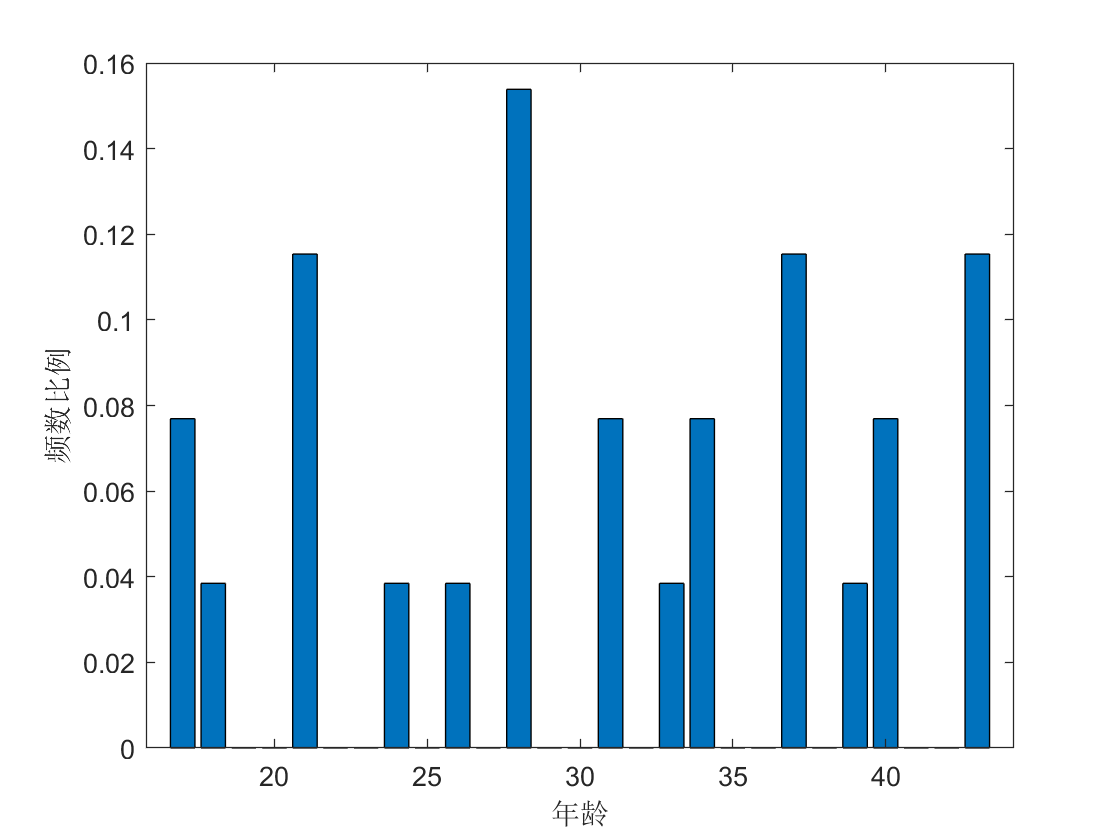
\includegraphics[width=1\textwidth]{figure/1.png}
        \end{minipage}
            \label{fig:2}
        } \\
        \subfigure[标题三]
        {
        \begin{minipage}[b]{0.45\textwidth}
        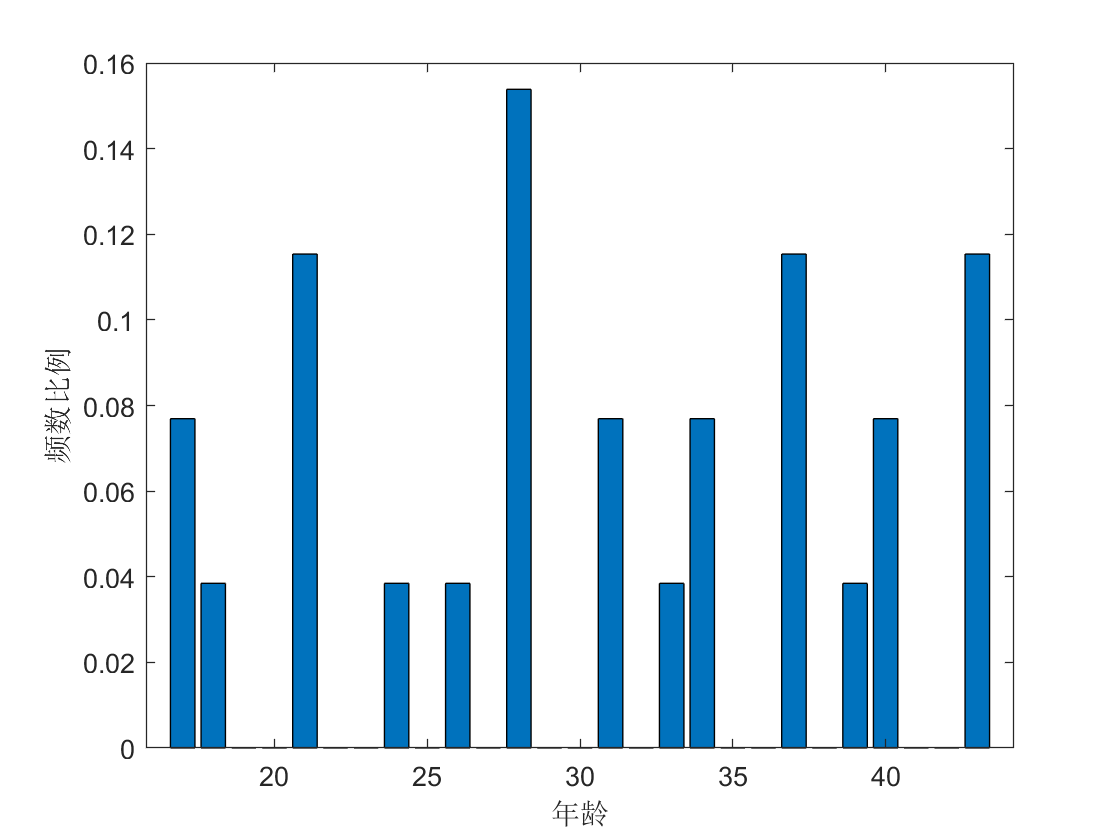
\includegraphics[width=1\textwidth]{figure/1.png}
        \end{minipage}
            \label{fig:3}
        }
        \subfigure[标题四]
        {
        \begin{minipage}[b]{0.45\textwidth}
        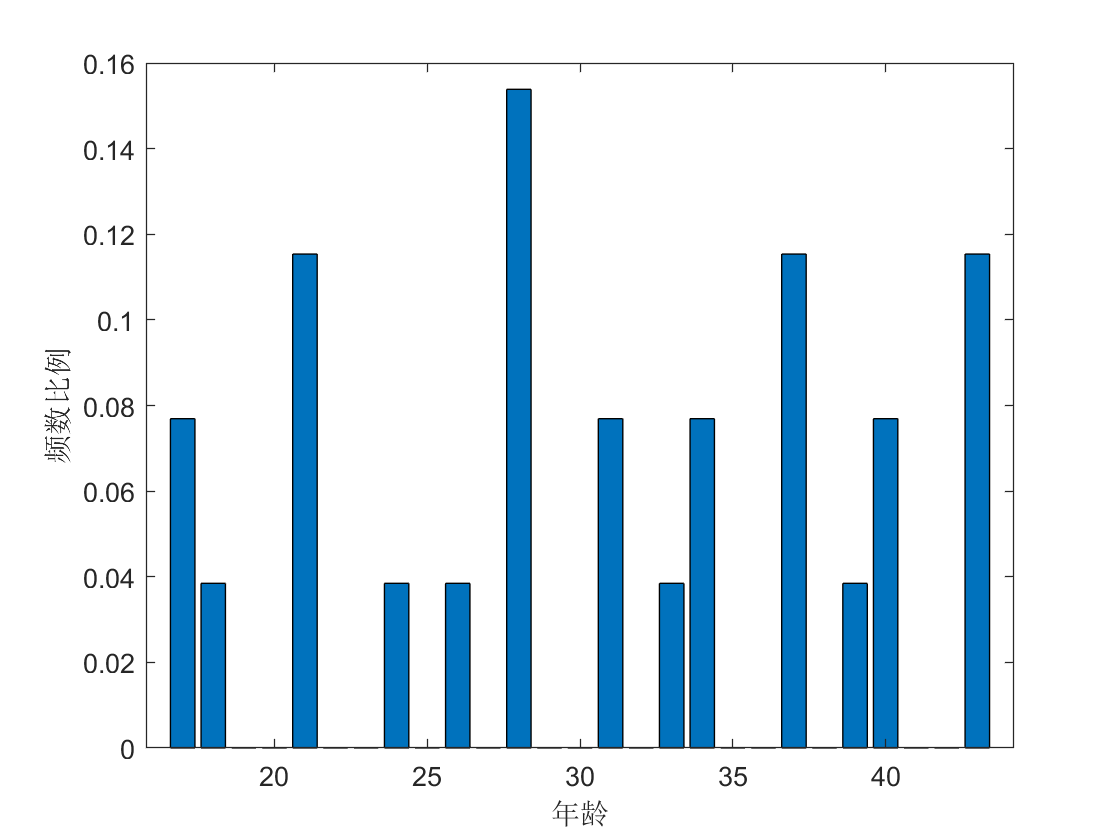
\includegraphics[width=1\textwidth]{figure/1.png}
        \end{minipage}
            \label{fig:4}
        }
        \caption{四图栅格布局摆放,统一大标题,独立子标题}
            \label{fig:5}
\end{figure}


这是子图\ref{fig:1}

这是子图\ref{fig:2}

这是子图\ref{fig:3}

这是子图\ref{fig:4}

这是大图\ref{fig:5}


\newpage
\section{表格}
\subsection{普通表格}
\begin{lstlisting}
%l:左对齐 c:居中对齐 r:右对齐(均指的是表格内文字)
%|表示竖直的表格线,\hline表示水平的表格线
%p{2.5cm}用于设置指定宽度的列,内容超过后自动换行
%hline水平线
% texdoc booktab(longtab tabu)查看更复杂的表格的制作
\begin{center}
    \begin{tabular}{|l|c|c|c|p{2.5cm}|}
    \hline
    姓名 & 语文 & 数学 & 外语 & 备注 \\
    \hline
    张三 & 87 & 100 & 93 & 优秀\\
    \hline
    李四 & 75 & 64 & 52 & 补考另行通知\\
    \hline
    王二 & 80 & 82 & 78 & 良好 \\
    \hline
\end{tabular}
\end{center}
\end{lstlisting}

%表格的制作以及排版
%l:左对齐 c:居中对齐 r:右对齐(均指的是表格内文字)
%|表示竖直的表格线,\hline表示水平的表格线
%p{2.5cm}用于设置指定宽度的列,内容超过后自动换行
%hline水平线
% texdoc booktab(longtab tabu)查看更复杂的表格的制作
\begin{center}
    \begin{tabular}{|l|c|c|c|p{2.5cm}|}
    \hline
    姓名 & 语文 & 数学 & 外语 & 备注 \\
    \hline
    张三 & 87 & 100 & 93 & 优秀\\
    \hline
    李四 & 75 & 64 & 52 & 补考另行通知\\
    \hline
    王二 & 80 & 82 & 78 & 良好 \\
    \hline
\end{tabular}
\end{center}

\subsubsection{三线表}
\subsubsection{添加宏包}
\begin{lstlisting}
\usepackage{booktabs}%提供命令\toprule、\midrule、\bottomrule
\end{lstlisting}

\subsubsection{案例}
\begin{lstlisting}
\begin{center}
\begin{tabular}{cc}
 \toprule[1.5pt]
 \makebox[0.3\textwidth][c]{符号}	&  \makebox[0.4\textwidth][c]{意义} \\
 \midrule[1pt]
 $ W $	    	& 某一小时内该路段运行总收益-总成本   \\ 
 $ W_0 $	        & 区分高峰和低峰的一个临界值  \\ 
 $ P $	    	& 线路在一小时内所有站的总上车人数 \\ 
 $ x $	    	& 线路在一小时内的车辆数 \\  
 $ T_t $	        & 长期趋势项 \\ 
 $ M_t $	        & 简单移动平均项 \\ 
\bottomrule[1.5pt]
\end{tabular}
\end{center}
\end{lstlisting}

\begin{center}
\begin{tabular}{cc}
 \toprule[1.5pt]
 \makebox[0.3\textwidth][c]{符号}	&  \makebox[0.4\textwidth][c]{意义} \\
 \midrule[1pt]
 $ W $	    	& 某一小时内该路段运行总收益-总成本   \\ 
 $ W_0 $	        & 区分高峰和低峰的一个临界值  \\ 
 $ P $	    	& 线路在一小时内所有站的总上车人数 \\ 
 $ x $	    	& 线路在一小时内的车辆数 \\  
 $ T_t $	        & 长期趋势项 \\ 
 $ M_t $	        & 简单移动平均项 \\ 
\bottomrule[1.5pt]
\end{tabular}
\end{center}

\subsection{进阶版}
\begin{lstlisting}
	\begin{center}
		\begin{tabular}{|c|c|c|c|}
			\hline
			& \multicolumn{3}{c|}{1} \\
			\hline
			7 & 5 &  & 3 \\
			\cline{1-2}
			\cline{4-4}
			1 & 6 & \multirow{2}{*}{2} & 8 \\
			\cline{1-2}
			\cline{4-4}
			9 & 2 &  & 4 \\
			\hline
		\end{tabular}
	\end{center}
\end{lstlisting}

\begin{center}
	\begin{tabular}{|c|c|c|c|}
		\hline
		& \multicolumn{3}{c|}{1} \\
		\hline
		7 & 5 &  & 3 \\
		\cline{1-2}
		\cline{4-4}
		1 & 6 & \multirow{2}{*}{2} & 8 \\
		\cline{1-2}
		\cline{4-4}
		9 & 2 &  & 4 \\
		\hline
	\end{tabular}
\end{center}

\begin{lstlisting}
	\begin{center}
		\begin{tabular}{|c|c|c|c|c|c|c|}
			\hline
			%前两行
			\multicolumn{7}{|c|}{\multirow{2}{*}{Central Topic} } \\
			\multicolumn{7}{|c|}{ } \\
			\hline
			%1
			\multicolumn{2}{|c|}{\multirow{6}{*}{Main Topic} } & \multirow{4}{*}{SubTopic}  & \multirow{3}{*}{SubTopic} & \multirow{2}{*}{SubTopic} & SubTopic & SubTopic \\
			\cline{6-7}
			%2
			\multicolumn{2}{|c|}{ }  &  &  &  & SubTopic & SubTopic  \\
			\cline{5-7}
			%3
			\multicolumn{2}{|c|}{ }  &  &  & SubTopic & \multicolumn{2}{c|}{SubTopic}  \\
			\cline{4-7}
			%4
			\multicolumn{2}{|c|}{ }  &  & SubTopic & \multicolumn{3}{c|}{SubTopic} \\
			\cline{3-7}
			%5
			\multicolumn{2}{|c|}{ }  & \multirow{2}{*}{SubTopic} & \multirow{2}{*}{SubTopic} & SubTopic & SubTopic & SubTopic \\
			\cline{5-7}
			%6
			\multicolumn{2}{|c|}{ }  &  &  & \multicolumn{3}{c|}{SubTopic}  \\
			\hline
		\end{tabular}
	\end{center}
\end{lstlisting}

\begin{center}
	\begin{tabular}{|c|c|c|c|c|c|c|}
		\hline
		%前两行
		\multicolumn{7}{|c|}{\multirow{2}{*}{Central Topic} } \\
		\multicolumn{7}{|c|}{ } \\
		\hline
		%1
		\multicolumn{2}{|c|}{\multirow{6}{*}{Main Topic} } & \multirow{4}{*}{SubTopic}  & \multirow{3}{*}{SubTopic} & \multirow{2}{*}{SubTopic} & SubTopic & SubTopic \\
		\cline{6-7}
		%2
		\multicolumn{2}{|c|}{ }  &  &  &  & SubTopic & SubTopic  \\
		\cline{5-7}
		%3
		\multicolumn{2}{|c|}{ }  &  &  & SubTopic & \multicolumn{2}{c|}{SubTopic}  \\
		\cline{4-7}
		%4
		\multicolumn{2}{|c|}{ }  &  & SubTopic & \multicolumn{3}{c|}{SubTopic} \\
		\cline{3-7}
		%5
		\multicolumn{2}{|c|}{ }  & \multirow{2}{*}{SubTopic} & \multirow{2}{*}{SubTopic} & SubTopic & SubTopic & SubTopic \\
		\cline{5-7}
		%6
		\multicolumn{2}{|c|}{ }  &  &  & \multicolumn{3}{c|}{SubTopic}  \\
		\hline
	\end{tabular}
\end{center}

\subsection{使用工具提高效率}
\subsubsection{使用Excel2Latex}
 打开工作表→点击文件→选项→加载项
    \begin{figure}[H]%开始引用图片环境,[h]为固定图片,防止图片乱跑
    \centering%使图片居中
    %插入图片的命令,[scale]为图片大小,后面跟着图片的路径和名字。也可以使用width和height更改图片的大小
    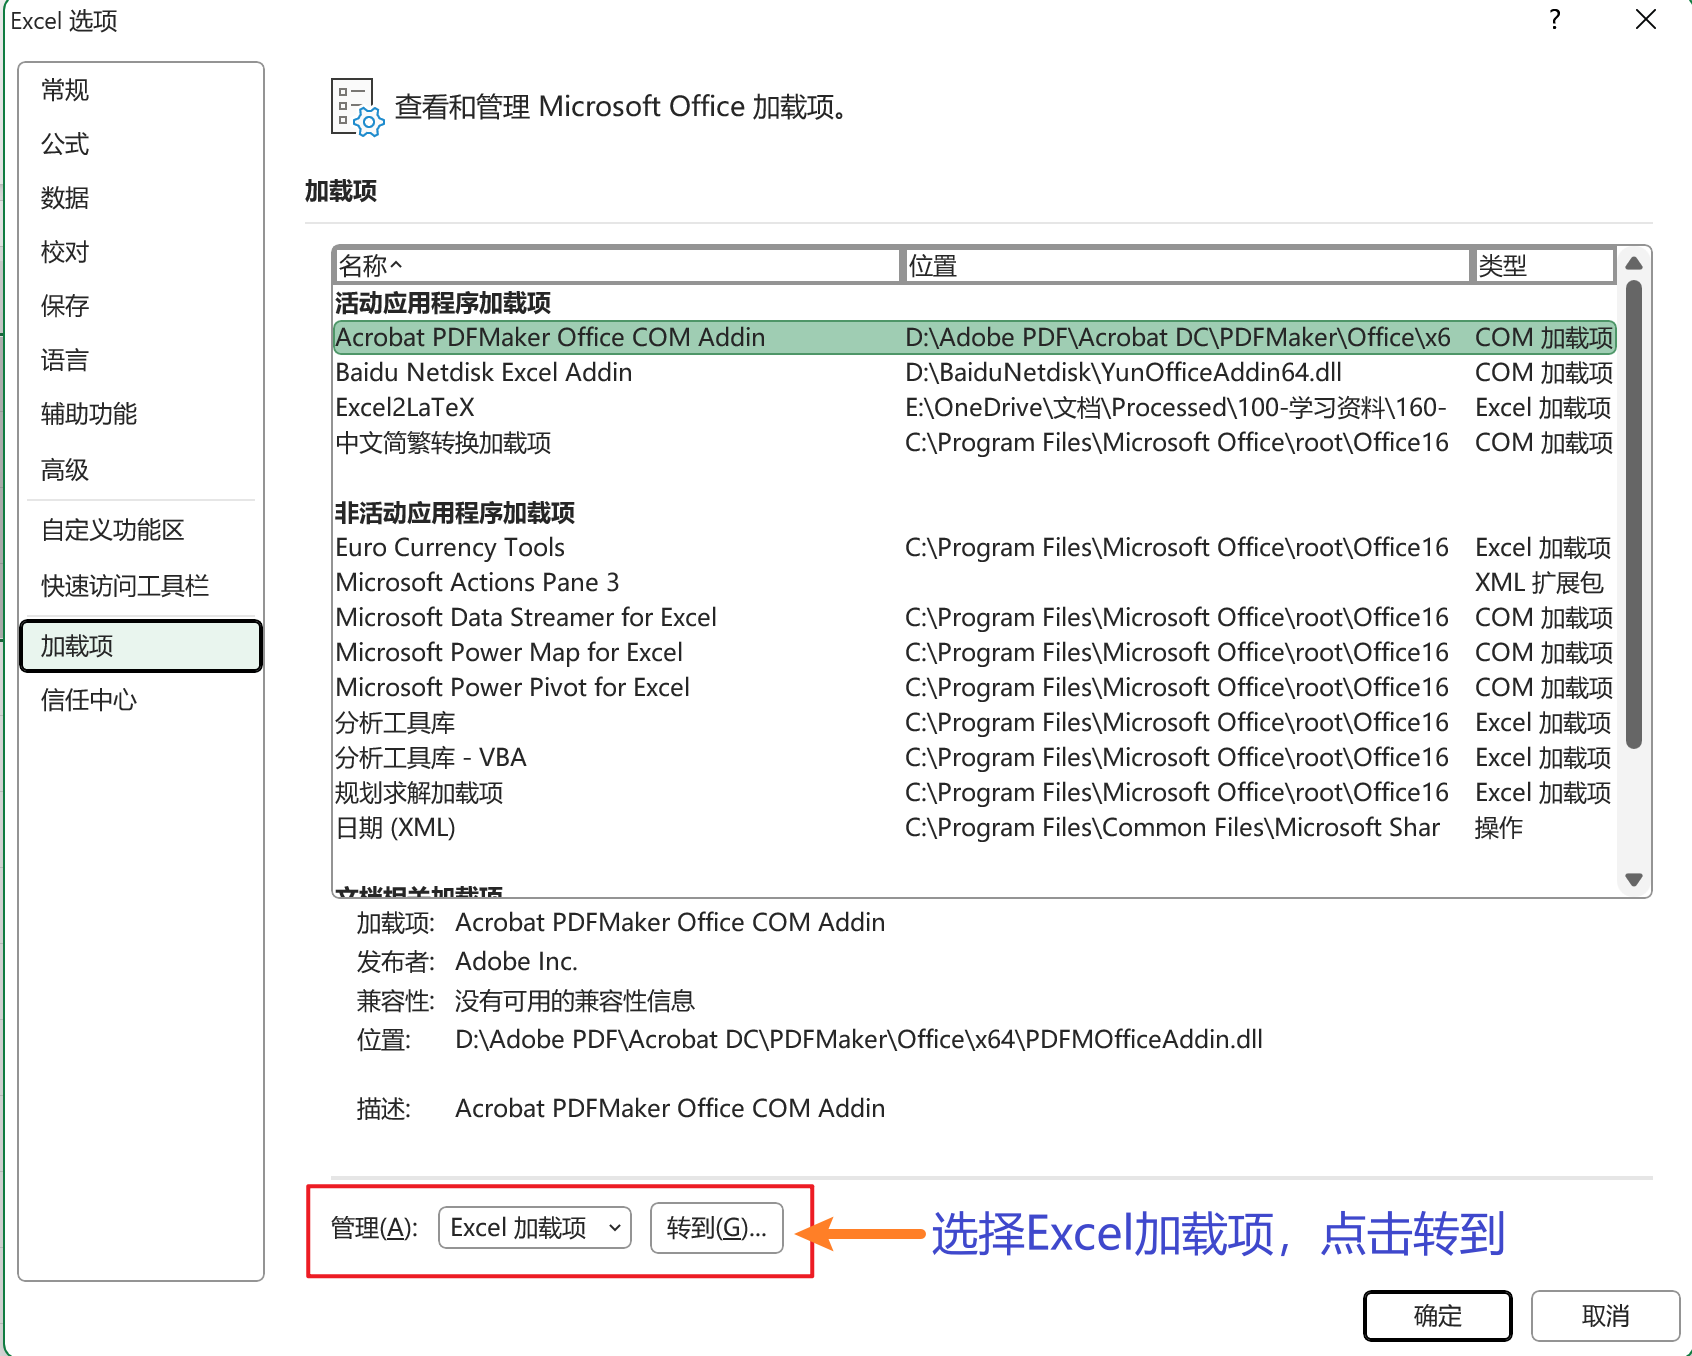
\includegraphics[width=14cm]{figure/2.png}
\end{figure}%结束引用图片环境

\begin{figure}[H]%开始引用图片环境,[h]为固定图片,防止图片乱跑
    \centering%使图片居中
    %插入图片的命令,[scale]为图片大小,后面跟着图片的路径和名字。也可以使用width和height更改图片的大小
    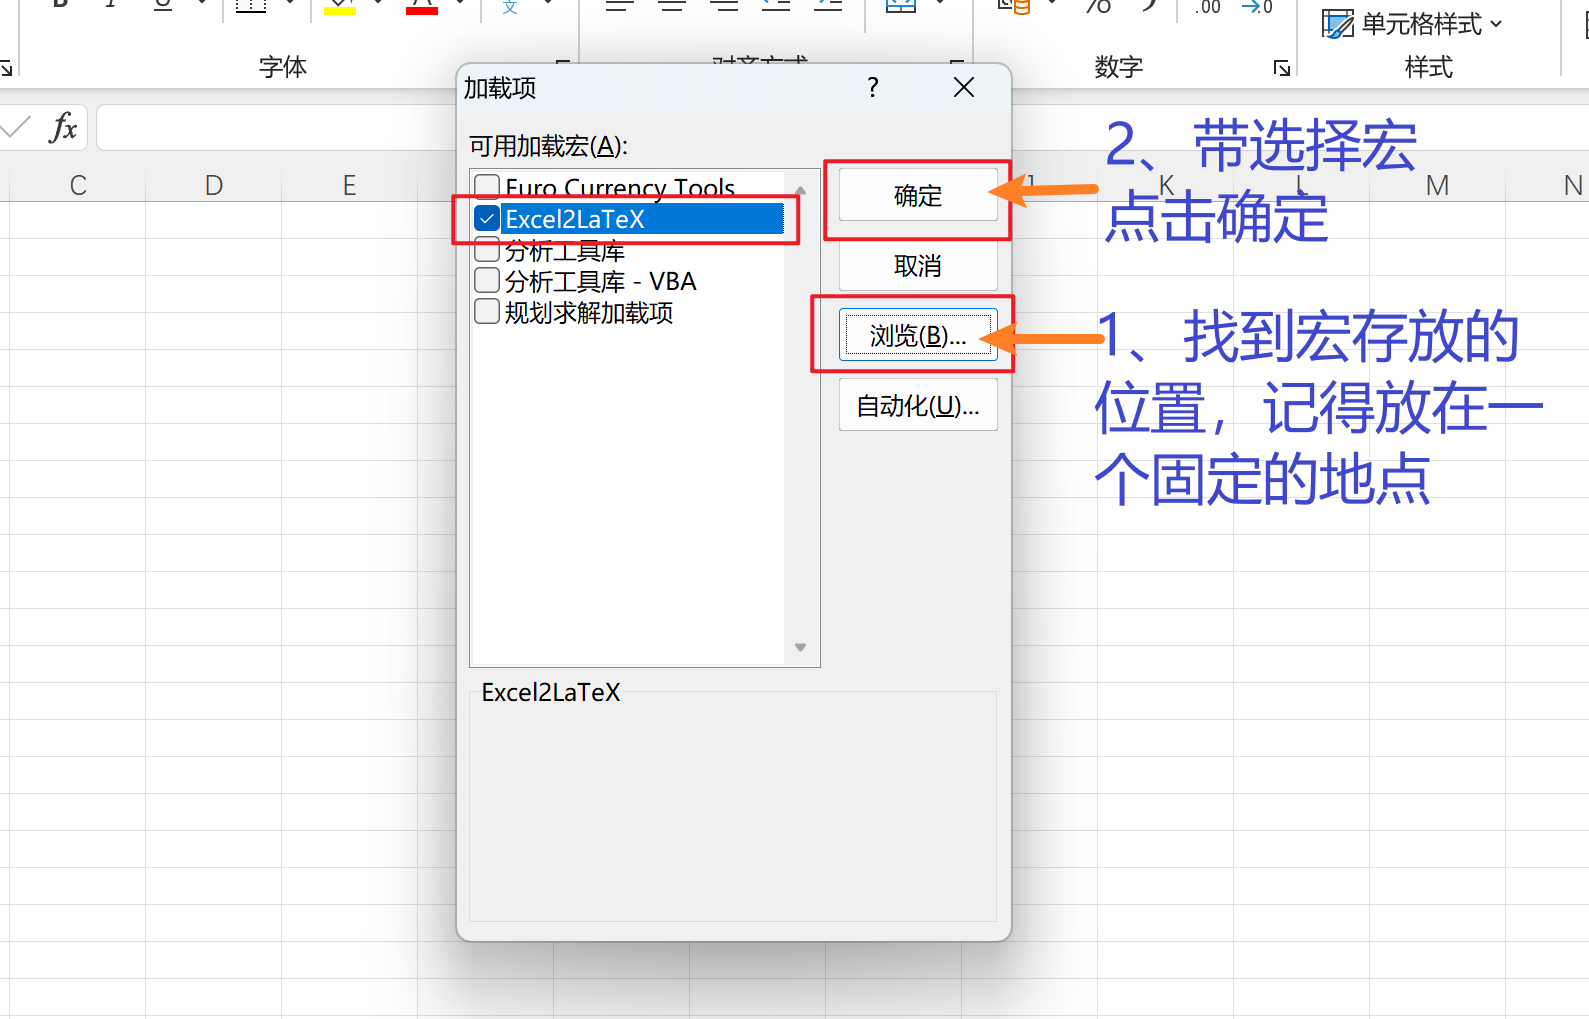
\includegraphics[width=14cm]{figure/3.png}
\end{figure}%结束引用图片环境
    
这样就加载进去了,以后也不用再次加载了。

不建议直接把宏直接拖进excle里面,因为office会检测到这是个有害的宏并删除,下次打开excle就要重新加载了。如下图所示:

\begin{figure}[H]%开始引用图片环境,[h]为固定图片,防止图片乱跑
    \centering%使图片居中
    %插入图片的命令,[scale]为图片大小,后面跟着图片的路径和名字。也可以使用width和height更改图片的大小
    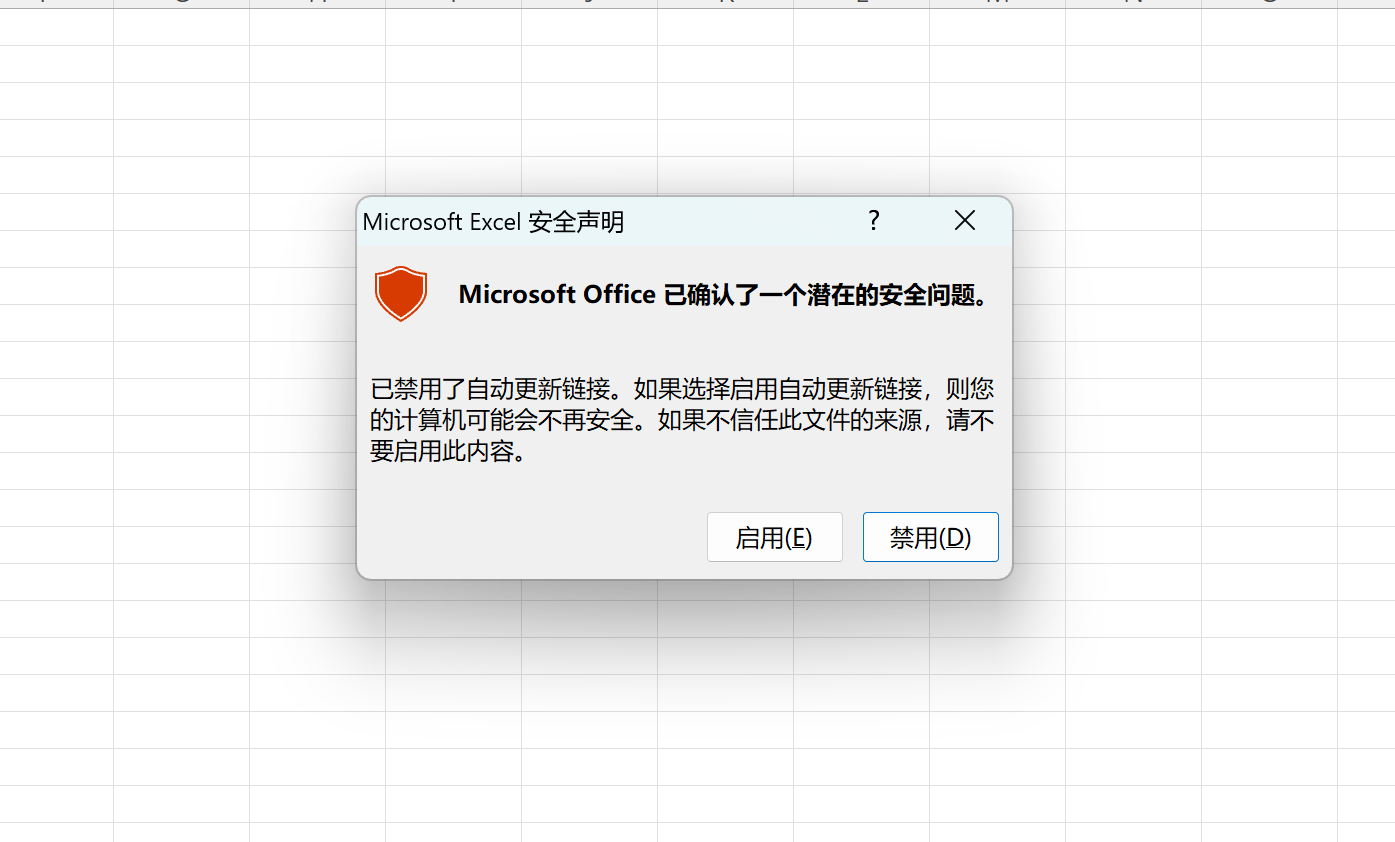
\includegraphics[width=16cm]{figure/4.png}
\end{figure}%结束引用图片环境

准备工作做好了之后就可以开始操作啦!

\begin{figure}[H]%开始引用图片环境,[h]为固定图片,防止图片乱跑
    \centering%使图片居中
    %插入图片的命令,[scale]为图片大小,后面跟着图片的路径和名字。也可以使用width和height更改图片的大小
    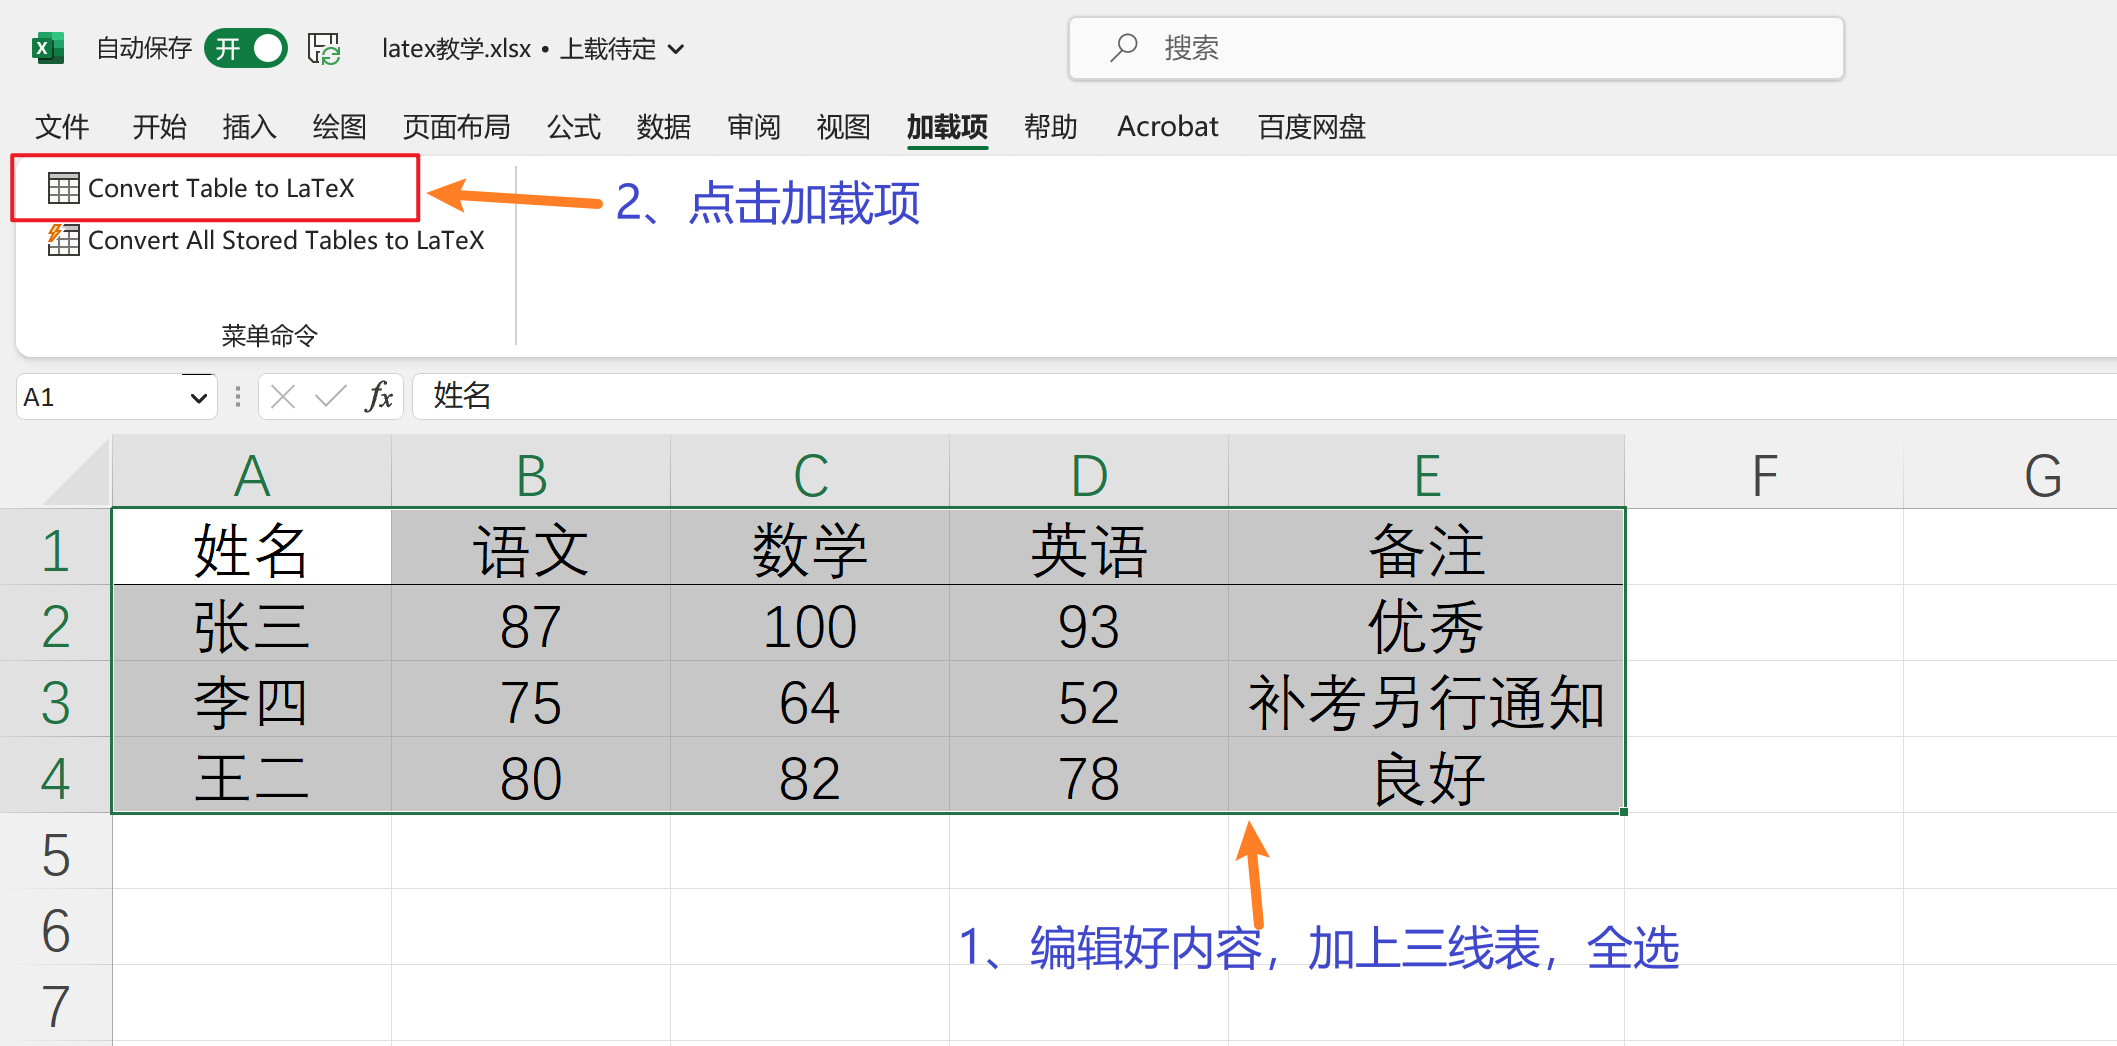
\includegraphics[width=16cm]{figure/5.png}
\end{figure}%结束引用图片环境

代码里会出现\lstinline{\bigstrut},需要添加宏包
\begin{lstlisting}
\usepackage{bigstrut}
\end{lstlisting}

\begin{figure}[H]%开始引用图片环境,[h]为固定图片,防止图片乱跑
    \centering%使图片居中
    %插入图片的命令,[scale]为图片大小,后面跟着图片的路径和名字。也可以使用width和height更改图片的大小
    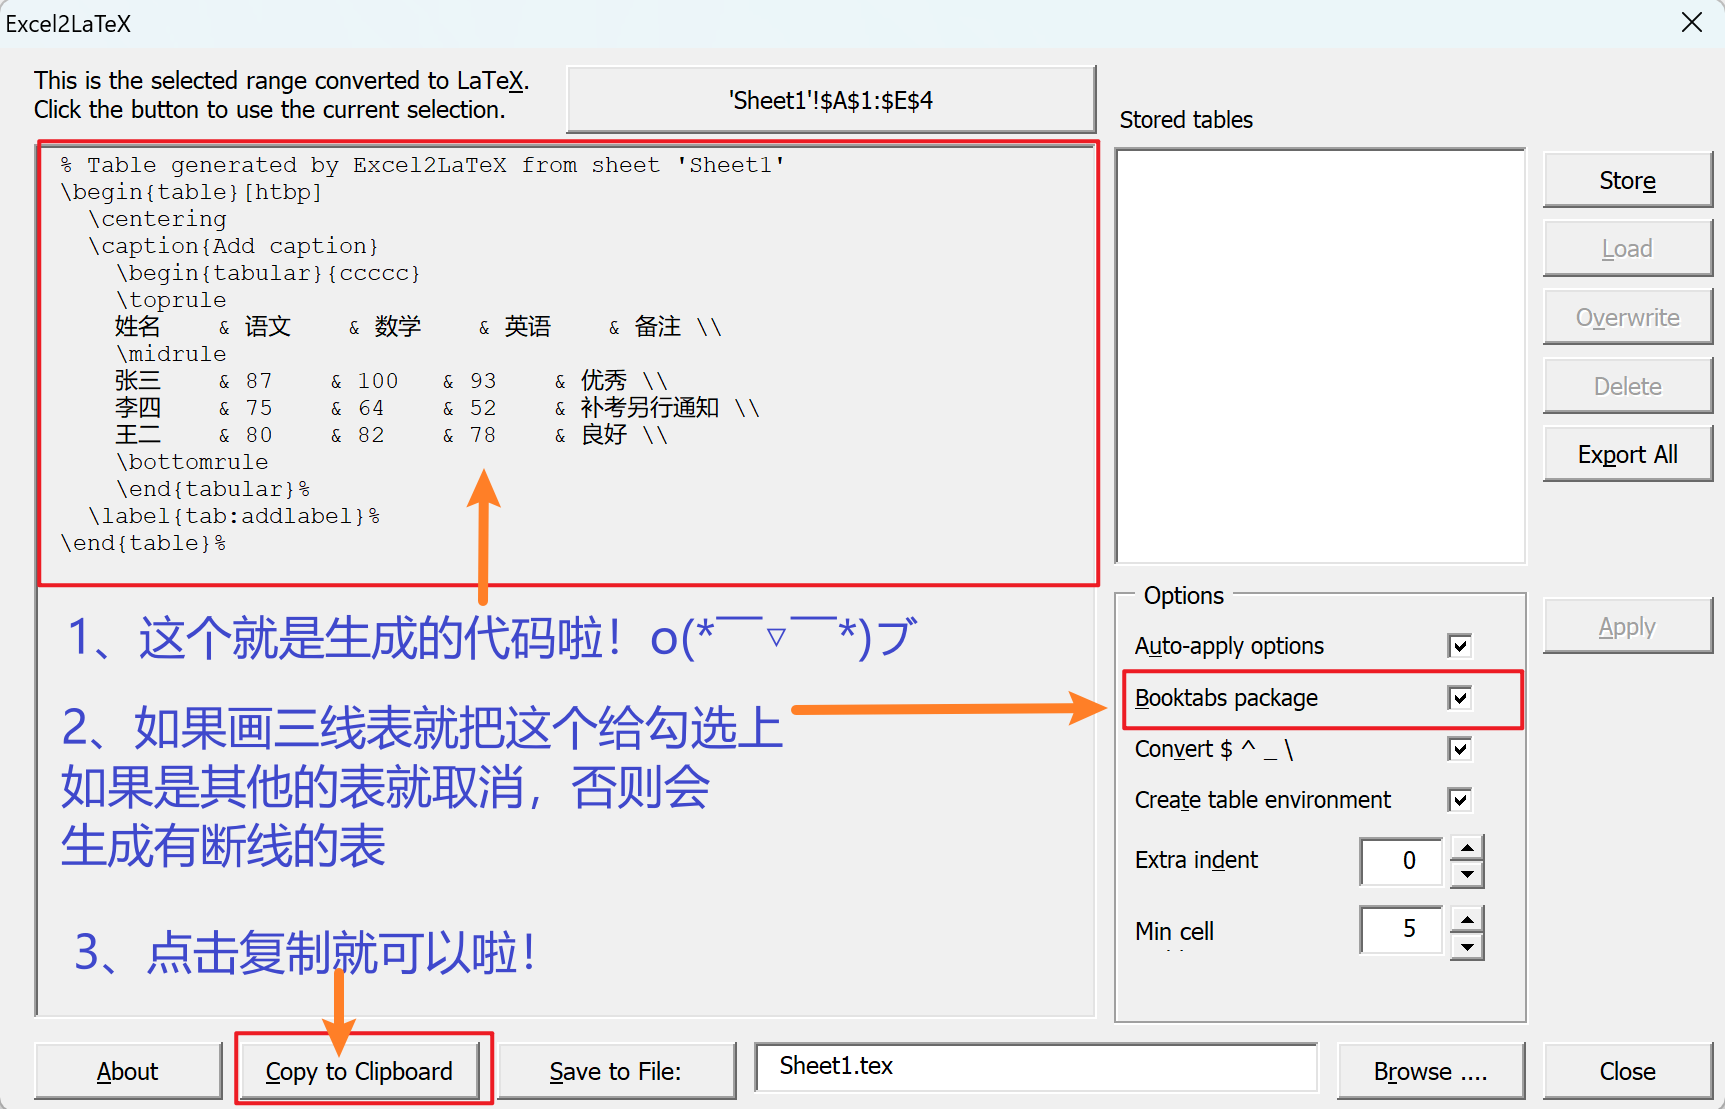
\includegraphics[width=16cm]{figure/6.png}
\end{figure}%结束引用图片环境

\subsubsection{使用Create LaTeX tables online}
\begin{figure}[H]%开始引用图片环境,[h]为固定图片,防止图片乱跑
    \centering%使图片居中
    %插入图片的命令,[scale]为图片大小,后面跟着图片的路径和名字。也可以使用width和height更改图片的大小
    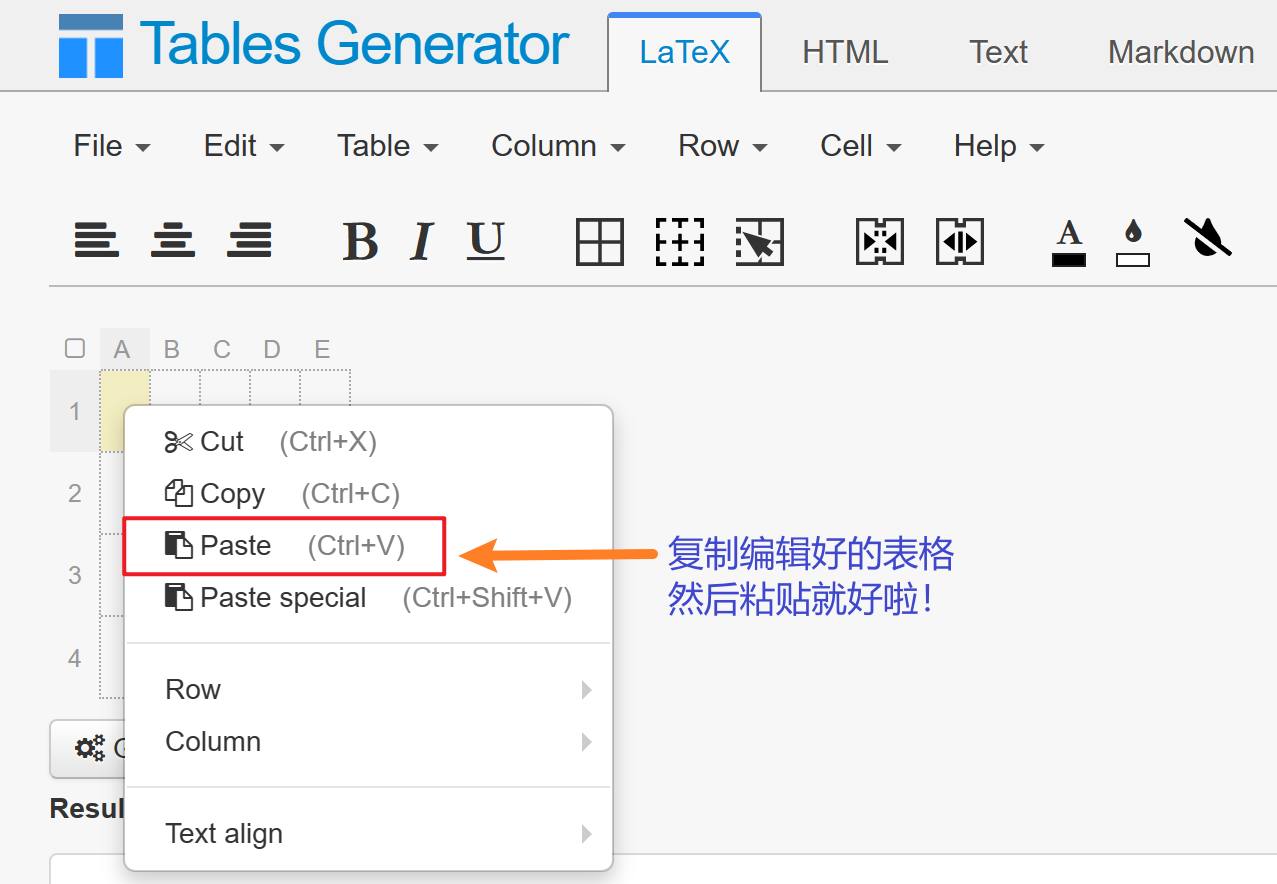
\includegraphics[width=16cm]{figure/7.png}
\end{figure}%结束引用图片环境

编辑表格并导出代码,再加上三线表的模板就好啦!
\begin{figure}[H]%开始引用图片环境,[h]为固定图片,防止图片乱跑
    \centering%使图片居中
    %插入图片的命令,[scale]为图片大小,后面跟着图片的路径和名字。也可以使用width和height更改图片的大小
    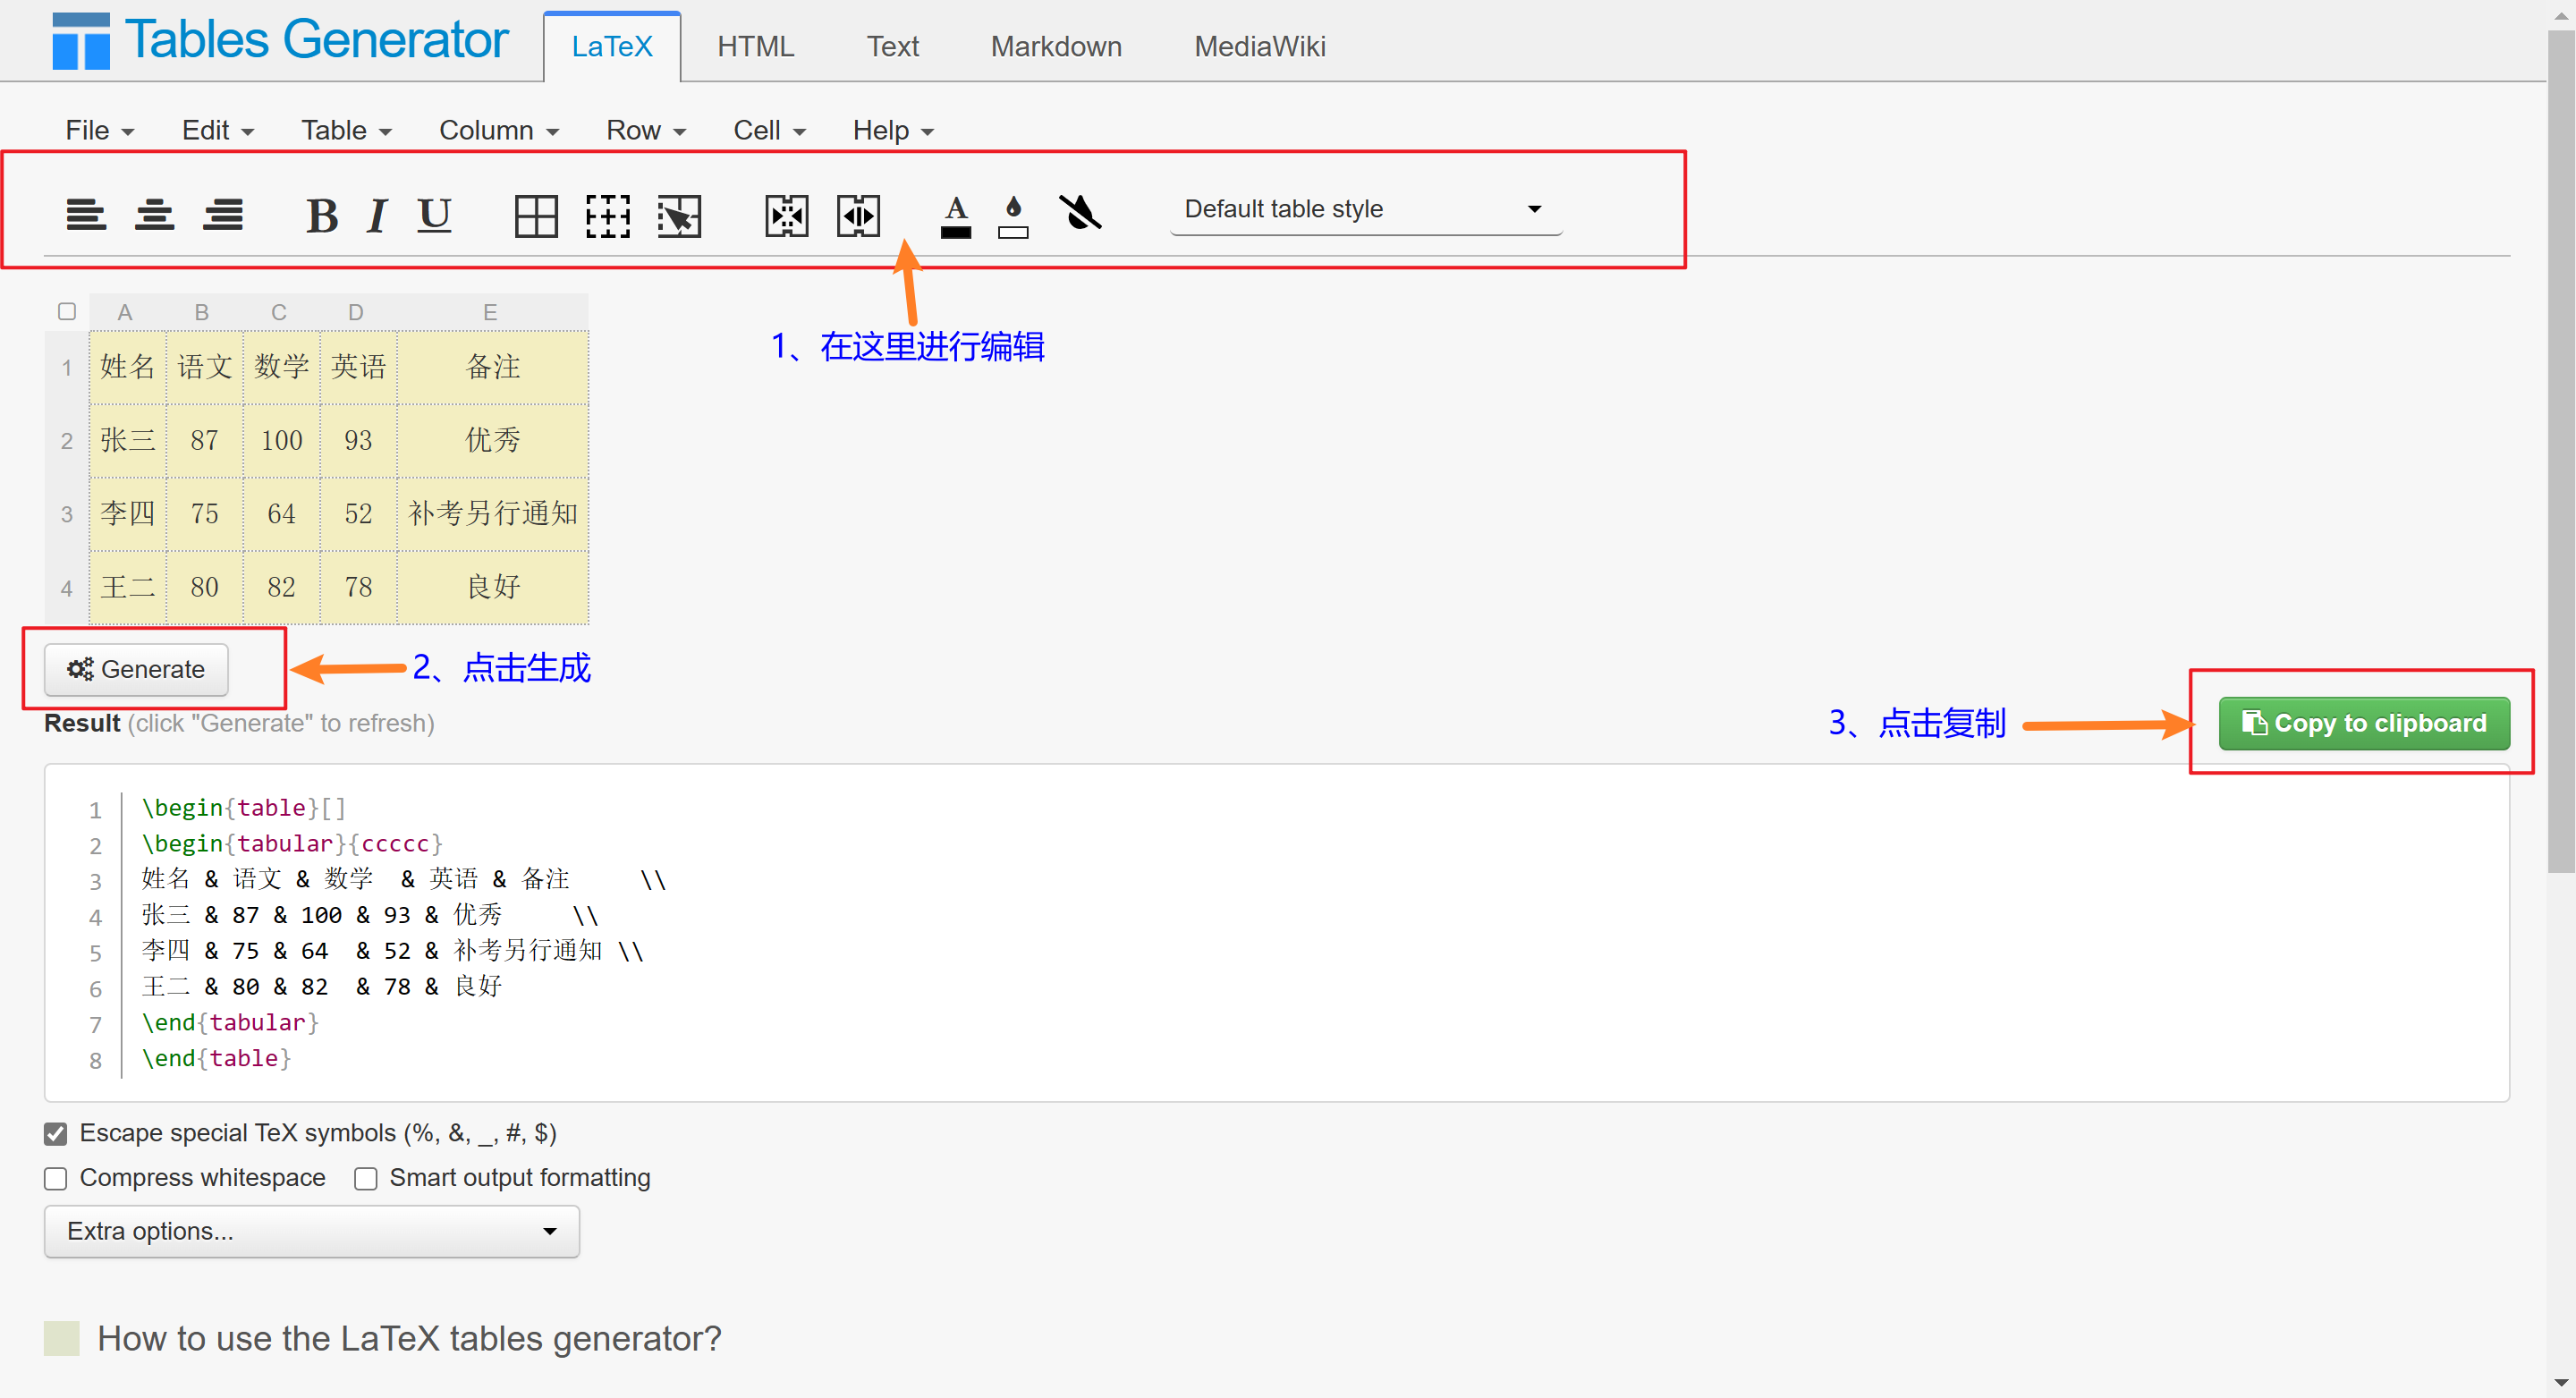
\includegraphics[width=15cm]{figure/8.png}
\end{figure}%结束引用图片环境


\section{代码}
\subsection{添加宏包}
\begin{lstlisting}
\usepackage{listings}
\end{lstlisting}

\subsection{进行代码环境的设置}
添加在cumcmthesis文件里,如果没有这个文件就添加在导言区。目的是使代码块更加美观。
\begin{lstlisting}
\lstset{numbers=left, %设置行号位置
        numberstyle=\scriptsize, %设置行号大小
        keywordstyle=\color{blue}, %设置关键字颜色
        commentstyle=\color[cmyk]{1,0,1,0}, %设置注释颜色
        frame=single, %设置边框格式
        escapeinside=``, %逃逸字符(1左面的键),用于显示中文
        breaklines, %自动折行
        extendedchars=true, %解决代码跨页时,章节标题,页眉等汉字不显示的问题
        xleftmargin=2em,xrightmargin=2em, aboveskip=1em, %设置边距
        tabsize=4, %设置tab空格数
        showspaces=false %不显示空格
\end{lstlisting}

\subsection{案例}
% \appendix %添加至\section{}前
\begin{lstlisting}[language=MATLAB]
function volume
%要求用户输入半径
r = input('输入半径:')
vol = (4/3)*pi*r^3;
disp('体积是:')
disp(vol)
\end{lstlisting}

\section{参考文献}
\subsection{普通方法}
去文献网站点击引用复制粘贴到LaTeX中

\begin{figure}[H]%开始引用图片环境,[h]为固定图片,防止图片乱跑
    \centering%使图片居中
    %插入图片的命令,[scale]为图片大小,后面跟着图片的路径和名字。也可以使用width和height更改图片的大小
    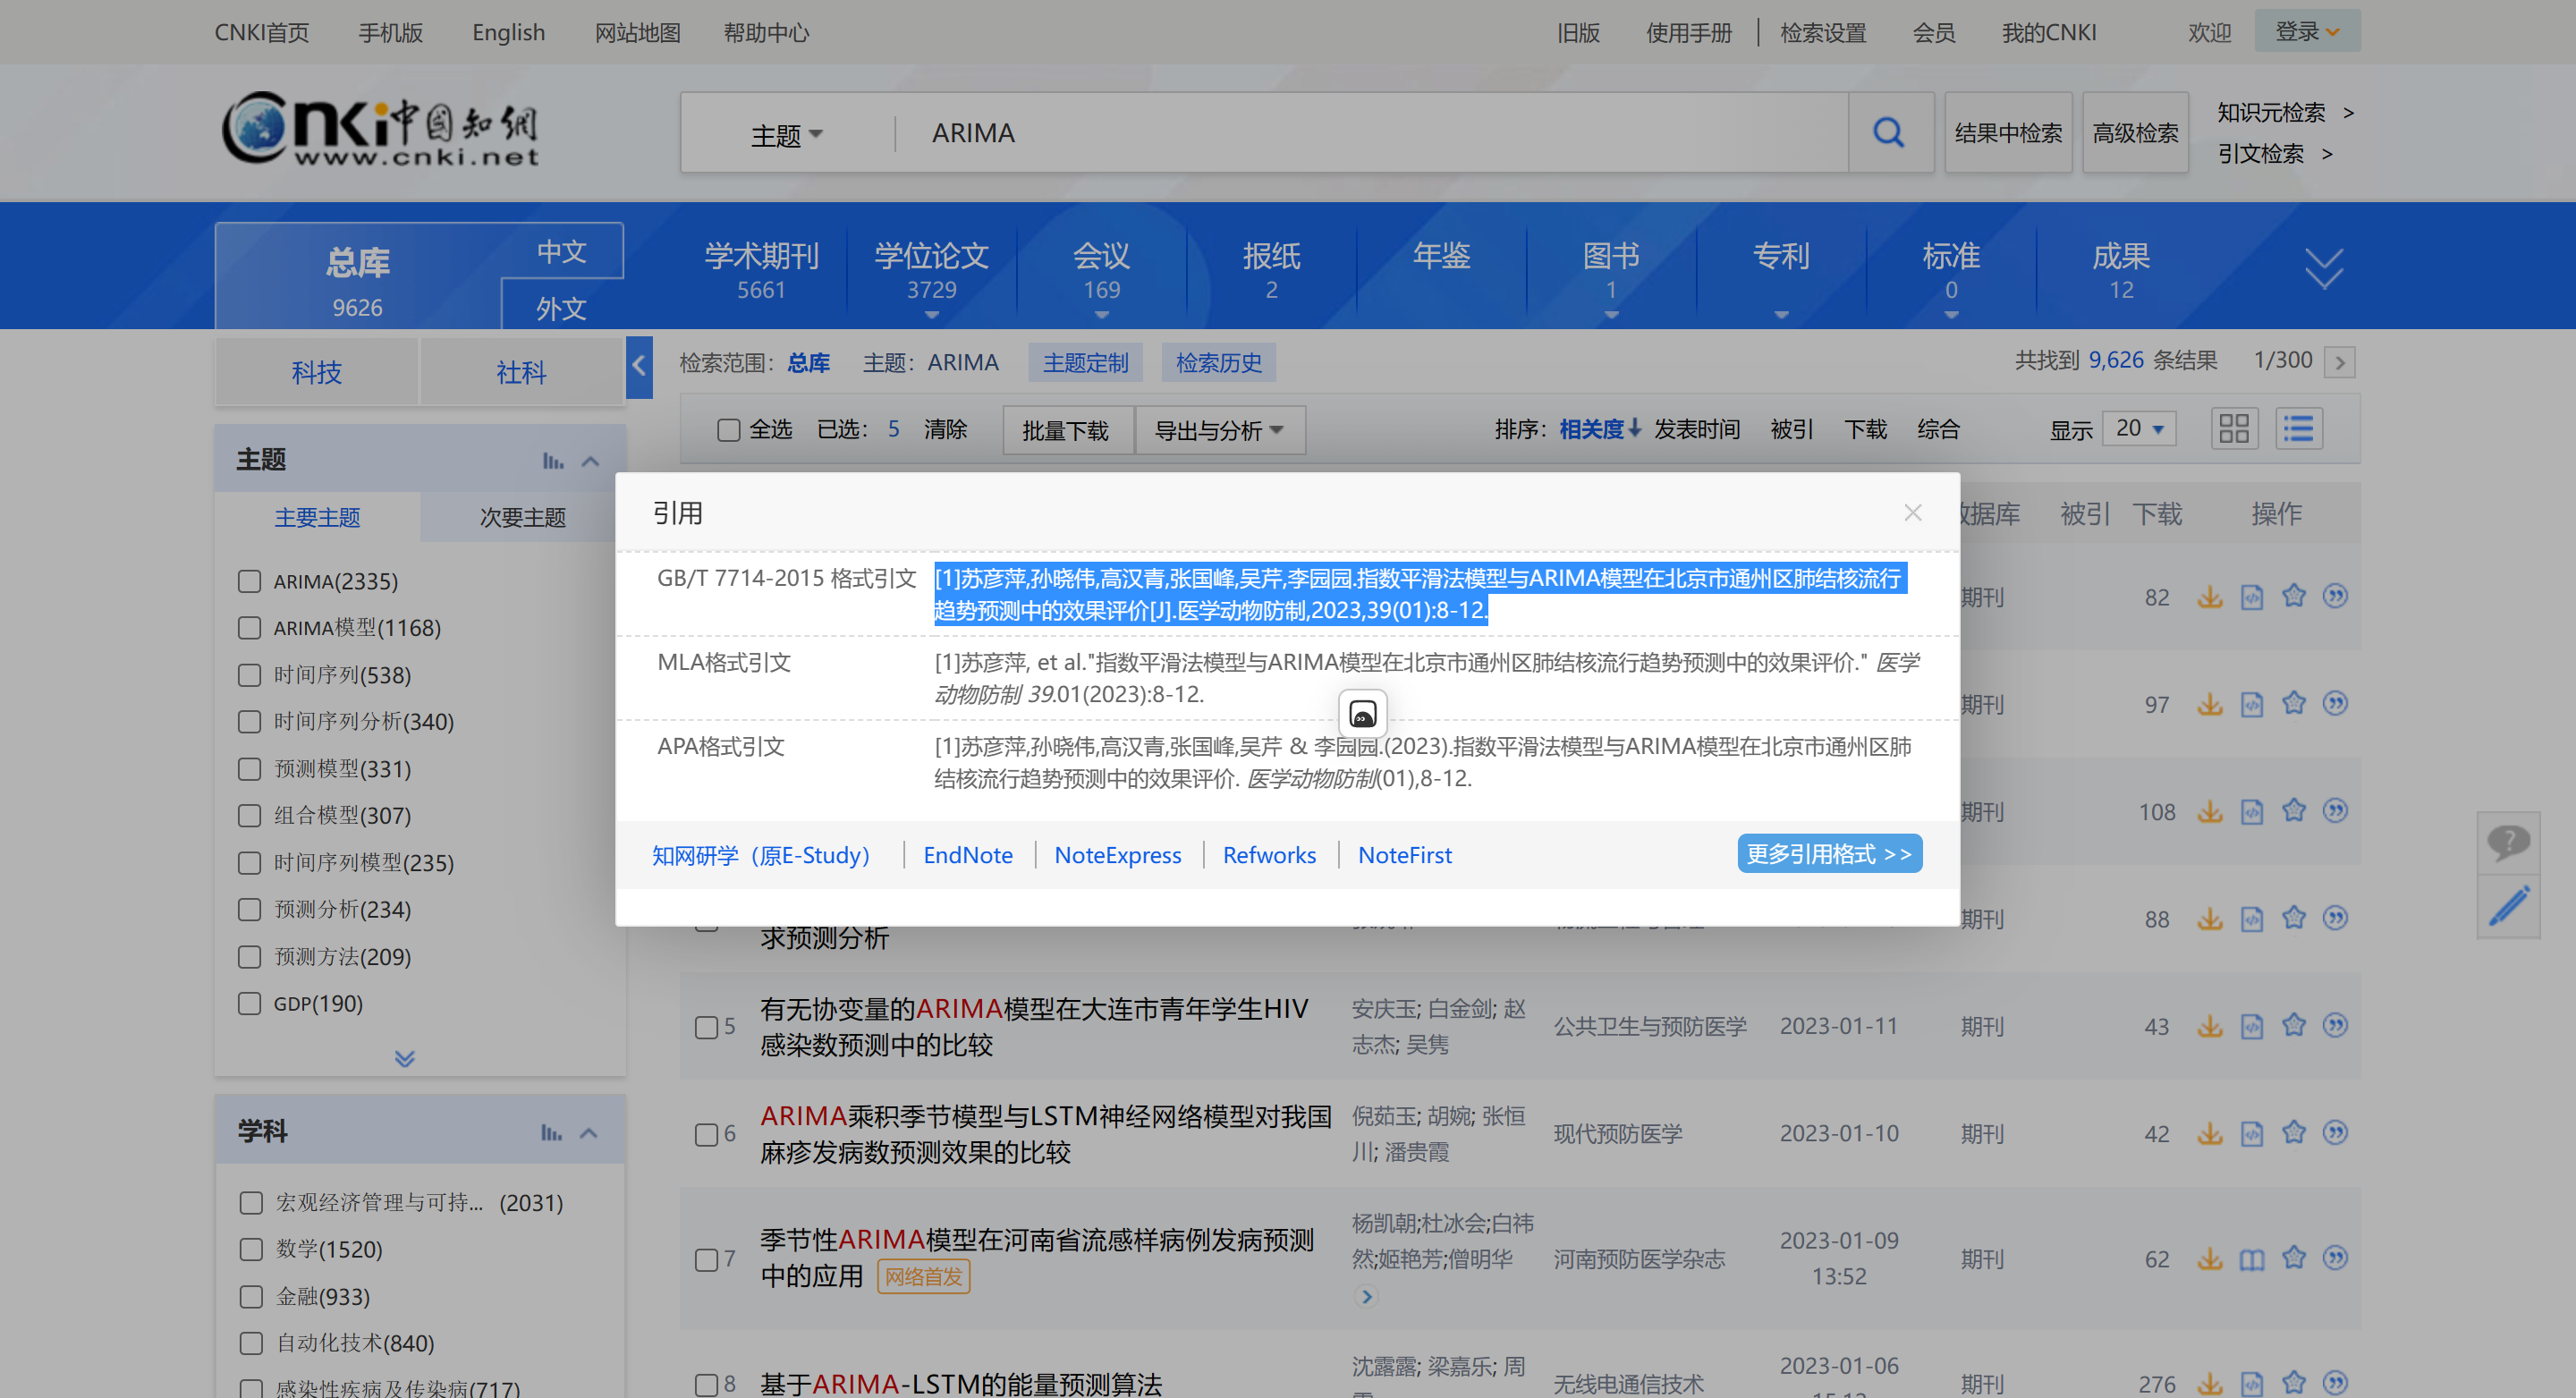
\includegraphics[width=14cm]{figure/9.png}
\end{figure}%结束引用图片环境

\begin{lstlisting}
引用一篇文章\textsuperscript{\cite{bib:1}}%引用方式
\begin{thebibliography}{9}%宽度9
    \bibitem{bib:1}%bib:1为标签,方便参考文献引用,引用:
    苏彦萍,孙晓伟,高汉青,张国峰,吴芹,李园园.指数平滑法模型与ARIMA模型在北京市通州区肺结核流行趋势预测中的效果评价[J].医学动物防制,2023,39(01):8-12.
\end {thebibliography}
\end{lstlisting}

引用一篇文章\textsuperscript{\cite{bib:1}}%引用方式
\begin{thebibliography}{9}%宽度9
    \bibitem{bib:1}%bib:1为标签,方便参考文献引用,引用:
    苏彦萍,孙晓伟,高汉青,张国峰,吴芹,李园园.指数平滑法模型与ARIMA模型在北京市通州区肺结核流行趋势预测中的效果评价[J].医学动物防制,2023,39(01):8-12.  
\end {thebibliography}

\subsection{自动导入方法}
\subsubsection{添加插件}
配合插件\href{https://github.com/l0o0/jasminum/releases}{jasminum}运行,之后要更改一下元数据的中英文转化,\href{https://www.bilibili.com/video/BV1F54y1k73n/?spm_id_from=333.1007.top_right_bar_window_history.content.click&vd_source=8ba9e5ab168044733acb427828b66aee}{Zotero 知网Translator 翻译器教程}

所有的基础设置都设置好就让我们开始吧!

\subsubsection{用Zotero保存文献}
使用Zotero插件

\begin{figure}[H]%开始引用图片环境,[h]为固定图片,防止图片乱跑
    \centering%使图片居中
    %插入图片的命令,[scale]为图片大小,后面跟着图片的路径和名字。也可以使用width和height更改图片的大小
    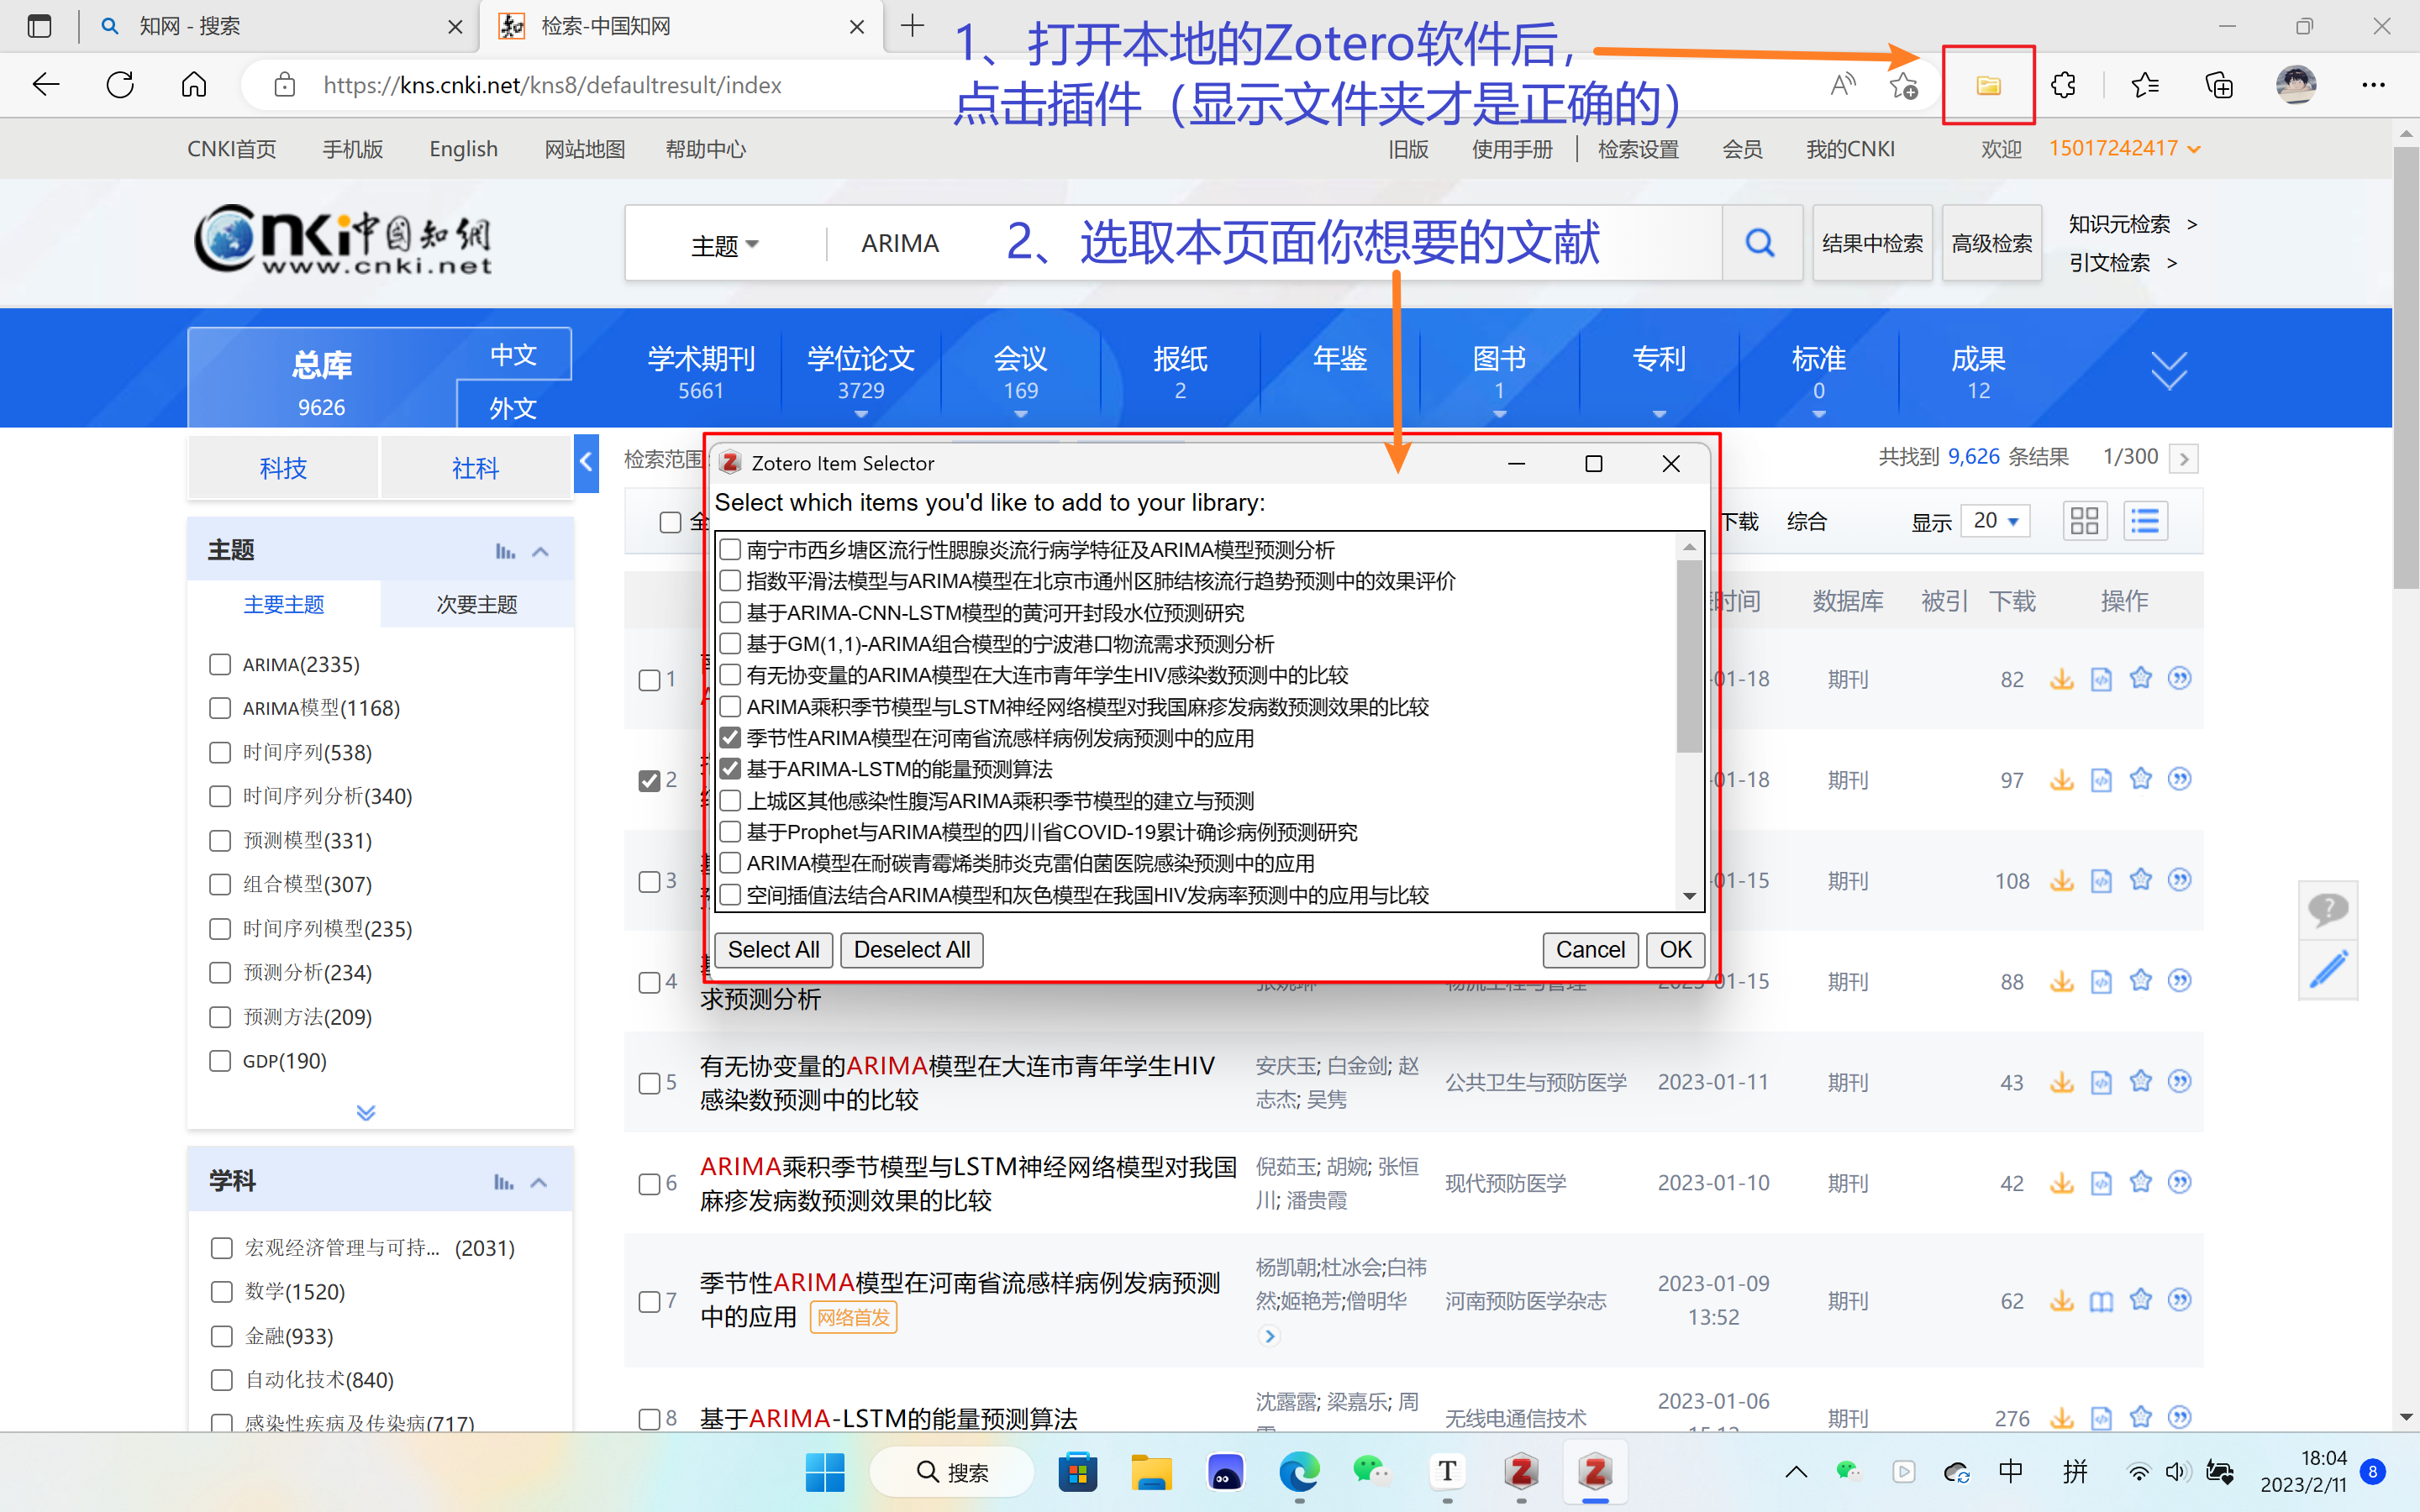
\includegraphics[width=16cm]{figure/10.png}
\end{figure}%结束引用图片环境

用茉莉花插件进行优化
\begin{figure}[H]%开始引用图片环境,[h]为固定图片,防止图片乱跑
    \centering%使图片居中
    %插入图片的命令,[scale]为图片大小,后面跟着图片的路径和名字。也可以使用width和height更改图片的大小
    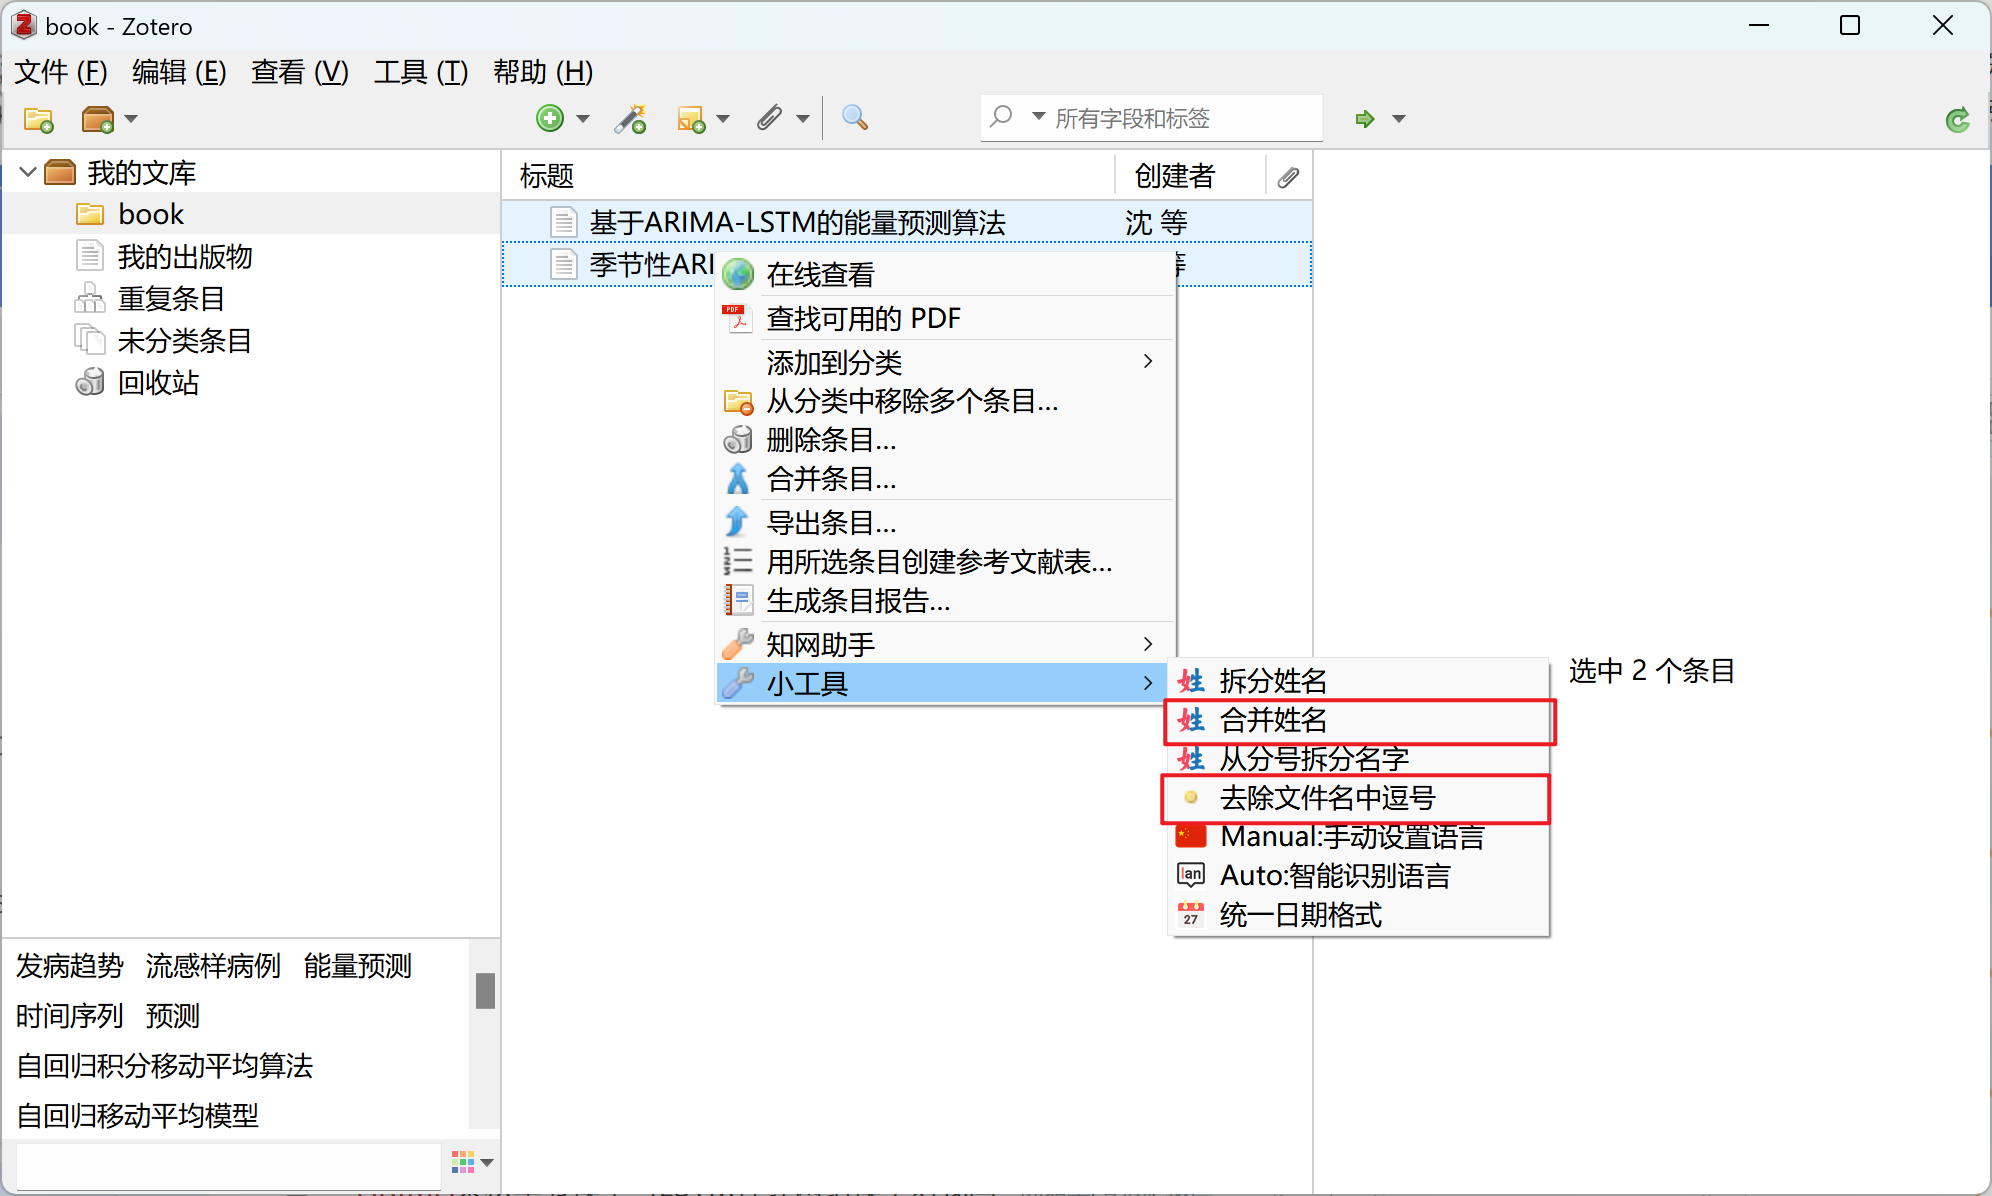
\includegraphics[width=16cm]{figure/11.png}
\end{figure}%结束引用图片环境

\subsubsection{导出bib文件并添加至LaTeX}
右键点击我的文库→导出文献库
\begin{figure}[H]%开始引用图片环境,[h]为固定图片,防止图片乱跑
    \centering%使图片居中
    %插入图片的命令,[scale]为图片大小,后面跟着图片的路径和名字。也可以使用width和height更改图片的大小
    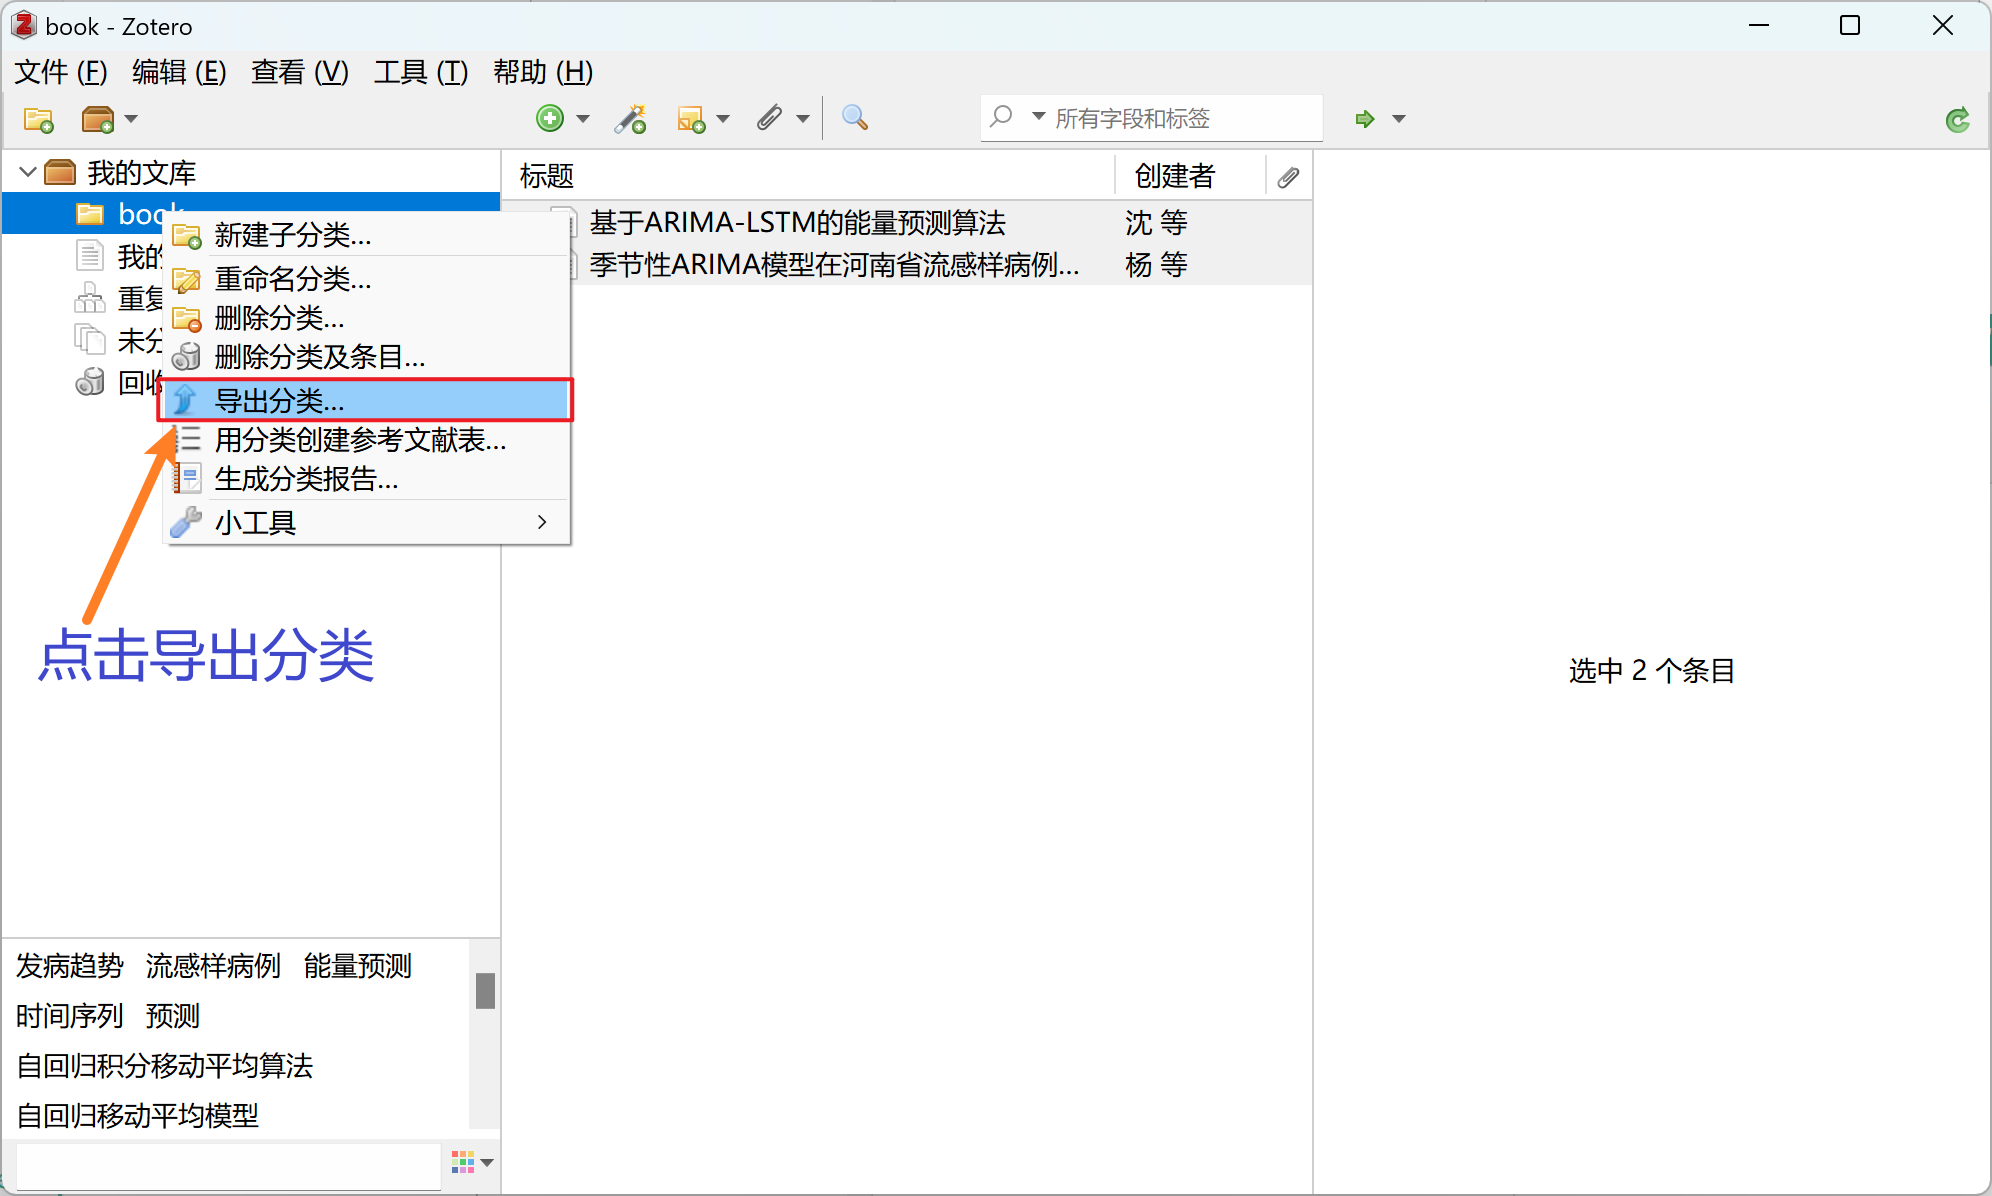
\includegraphics[width=16cm]{figure/12.png}
\end{figure}%结束引用图片环境

\newpage
导入bib文件
\begin{figure}[H]%开始引用图片环境,[h]为固定图片,防止图片乱跑
    \centering%使图片居中
    %插入图片的命令,[scale]为图片大小,后面跟着图片的路径和名字。也可以使用width和height更改图片的大小
    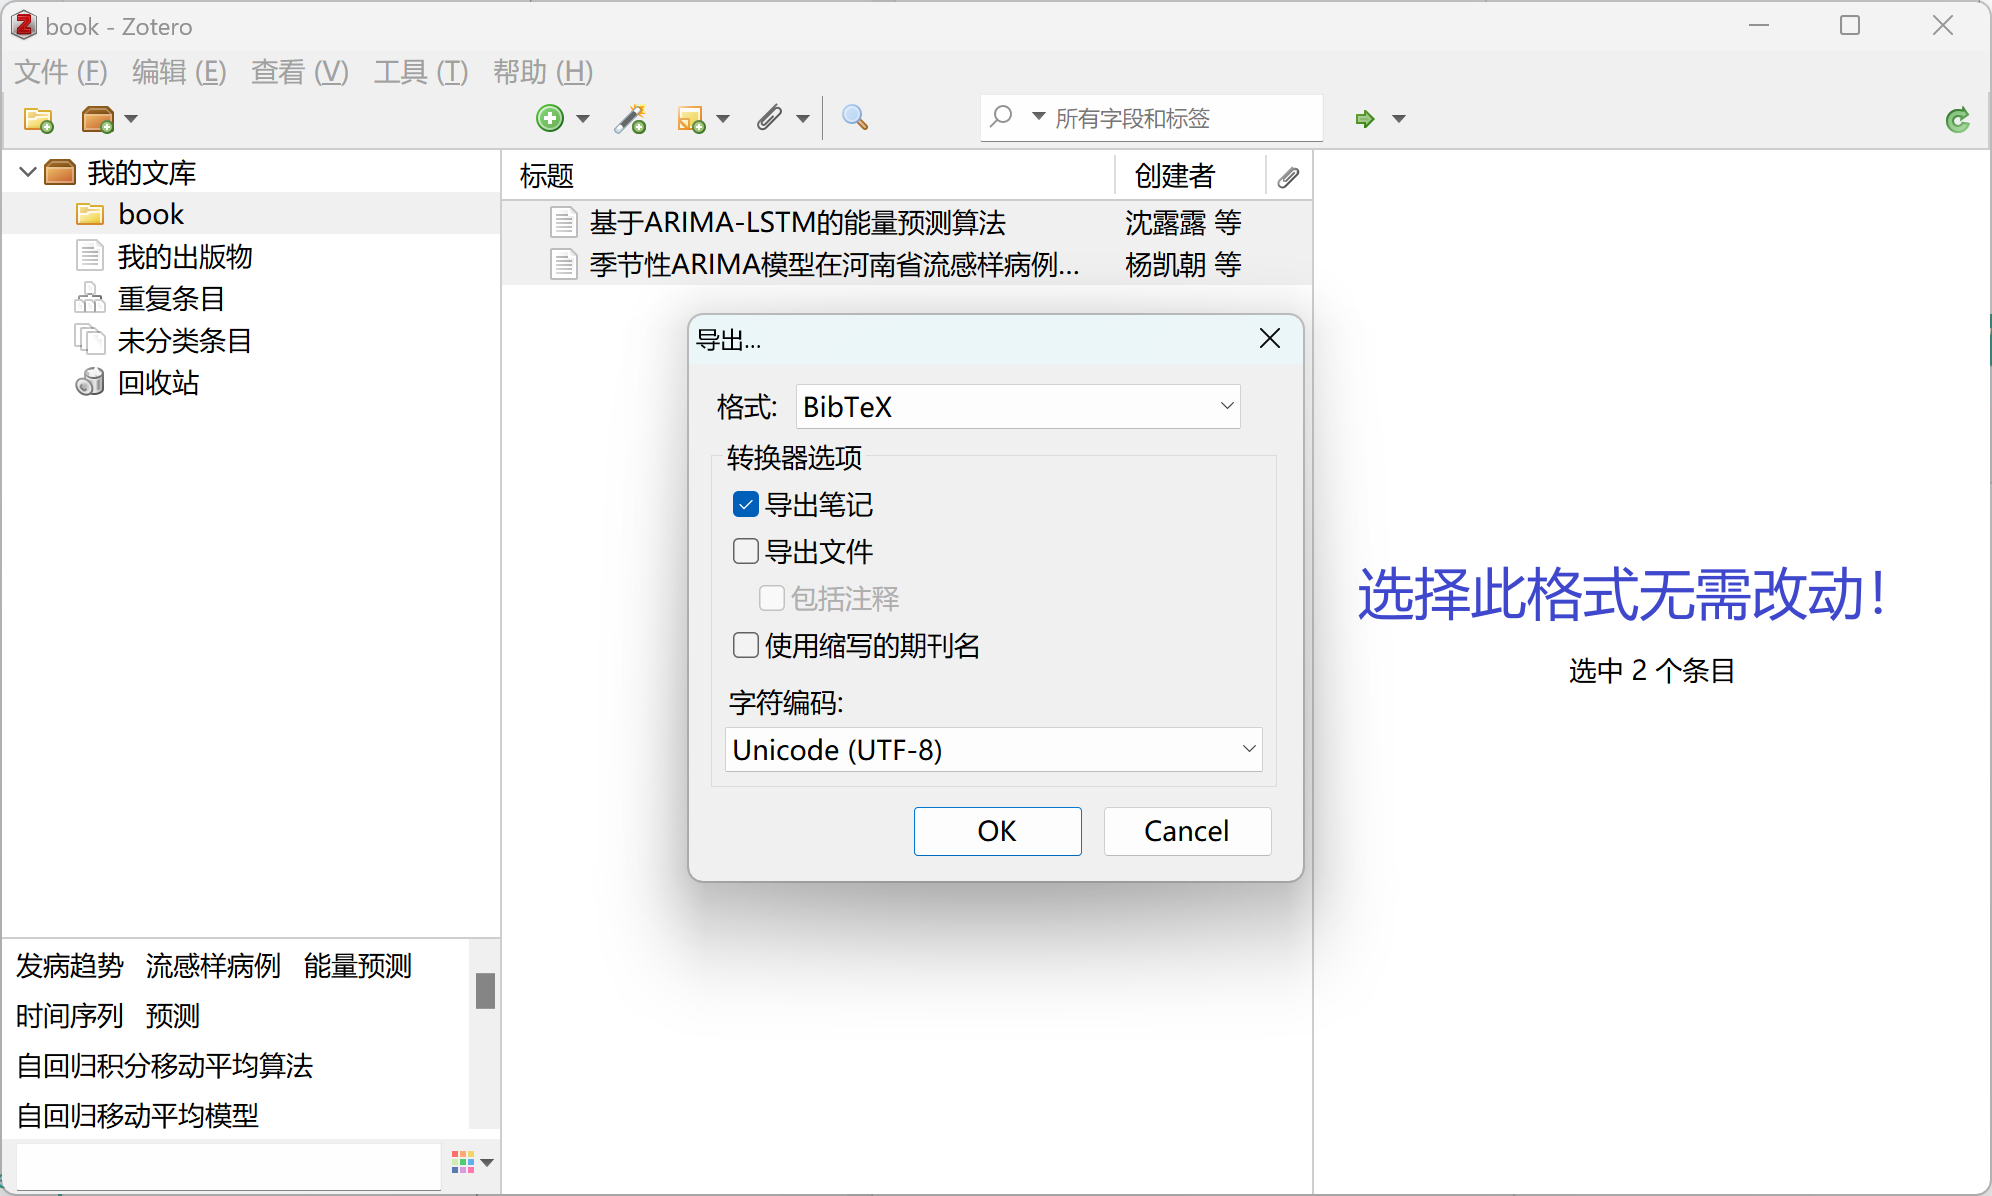
\includegraphics[width=16cm]{figure/13.png}
\end{figure}%结束引用图片环境

打开texpage上传文件
\begin{figure}[H]%开始引用图片环境,[h]为固定图片,防止图片乱跑
    \centering%使图片居中
    %插入图片的命令,[scale]为图片大小,后面跟着图片的路径和名字。也可以使用width和height更改图片的大小
    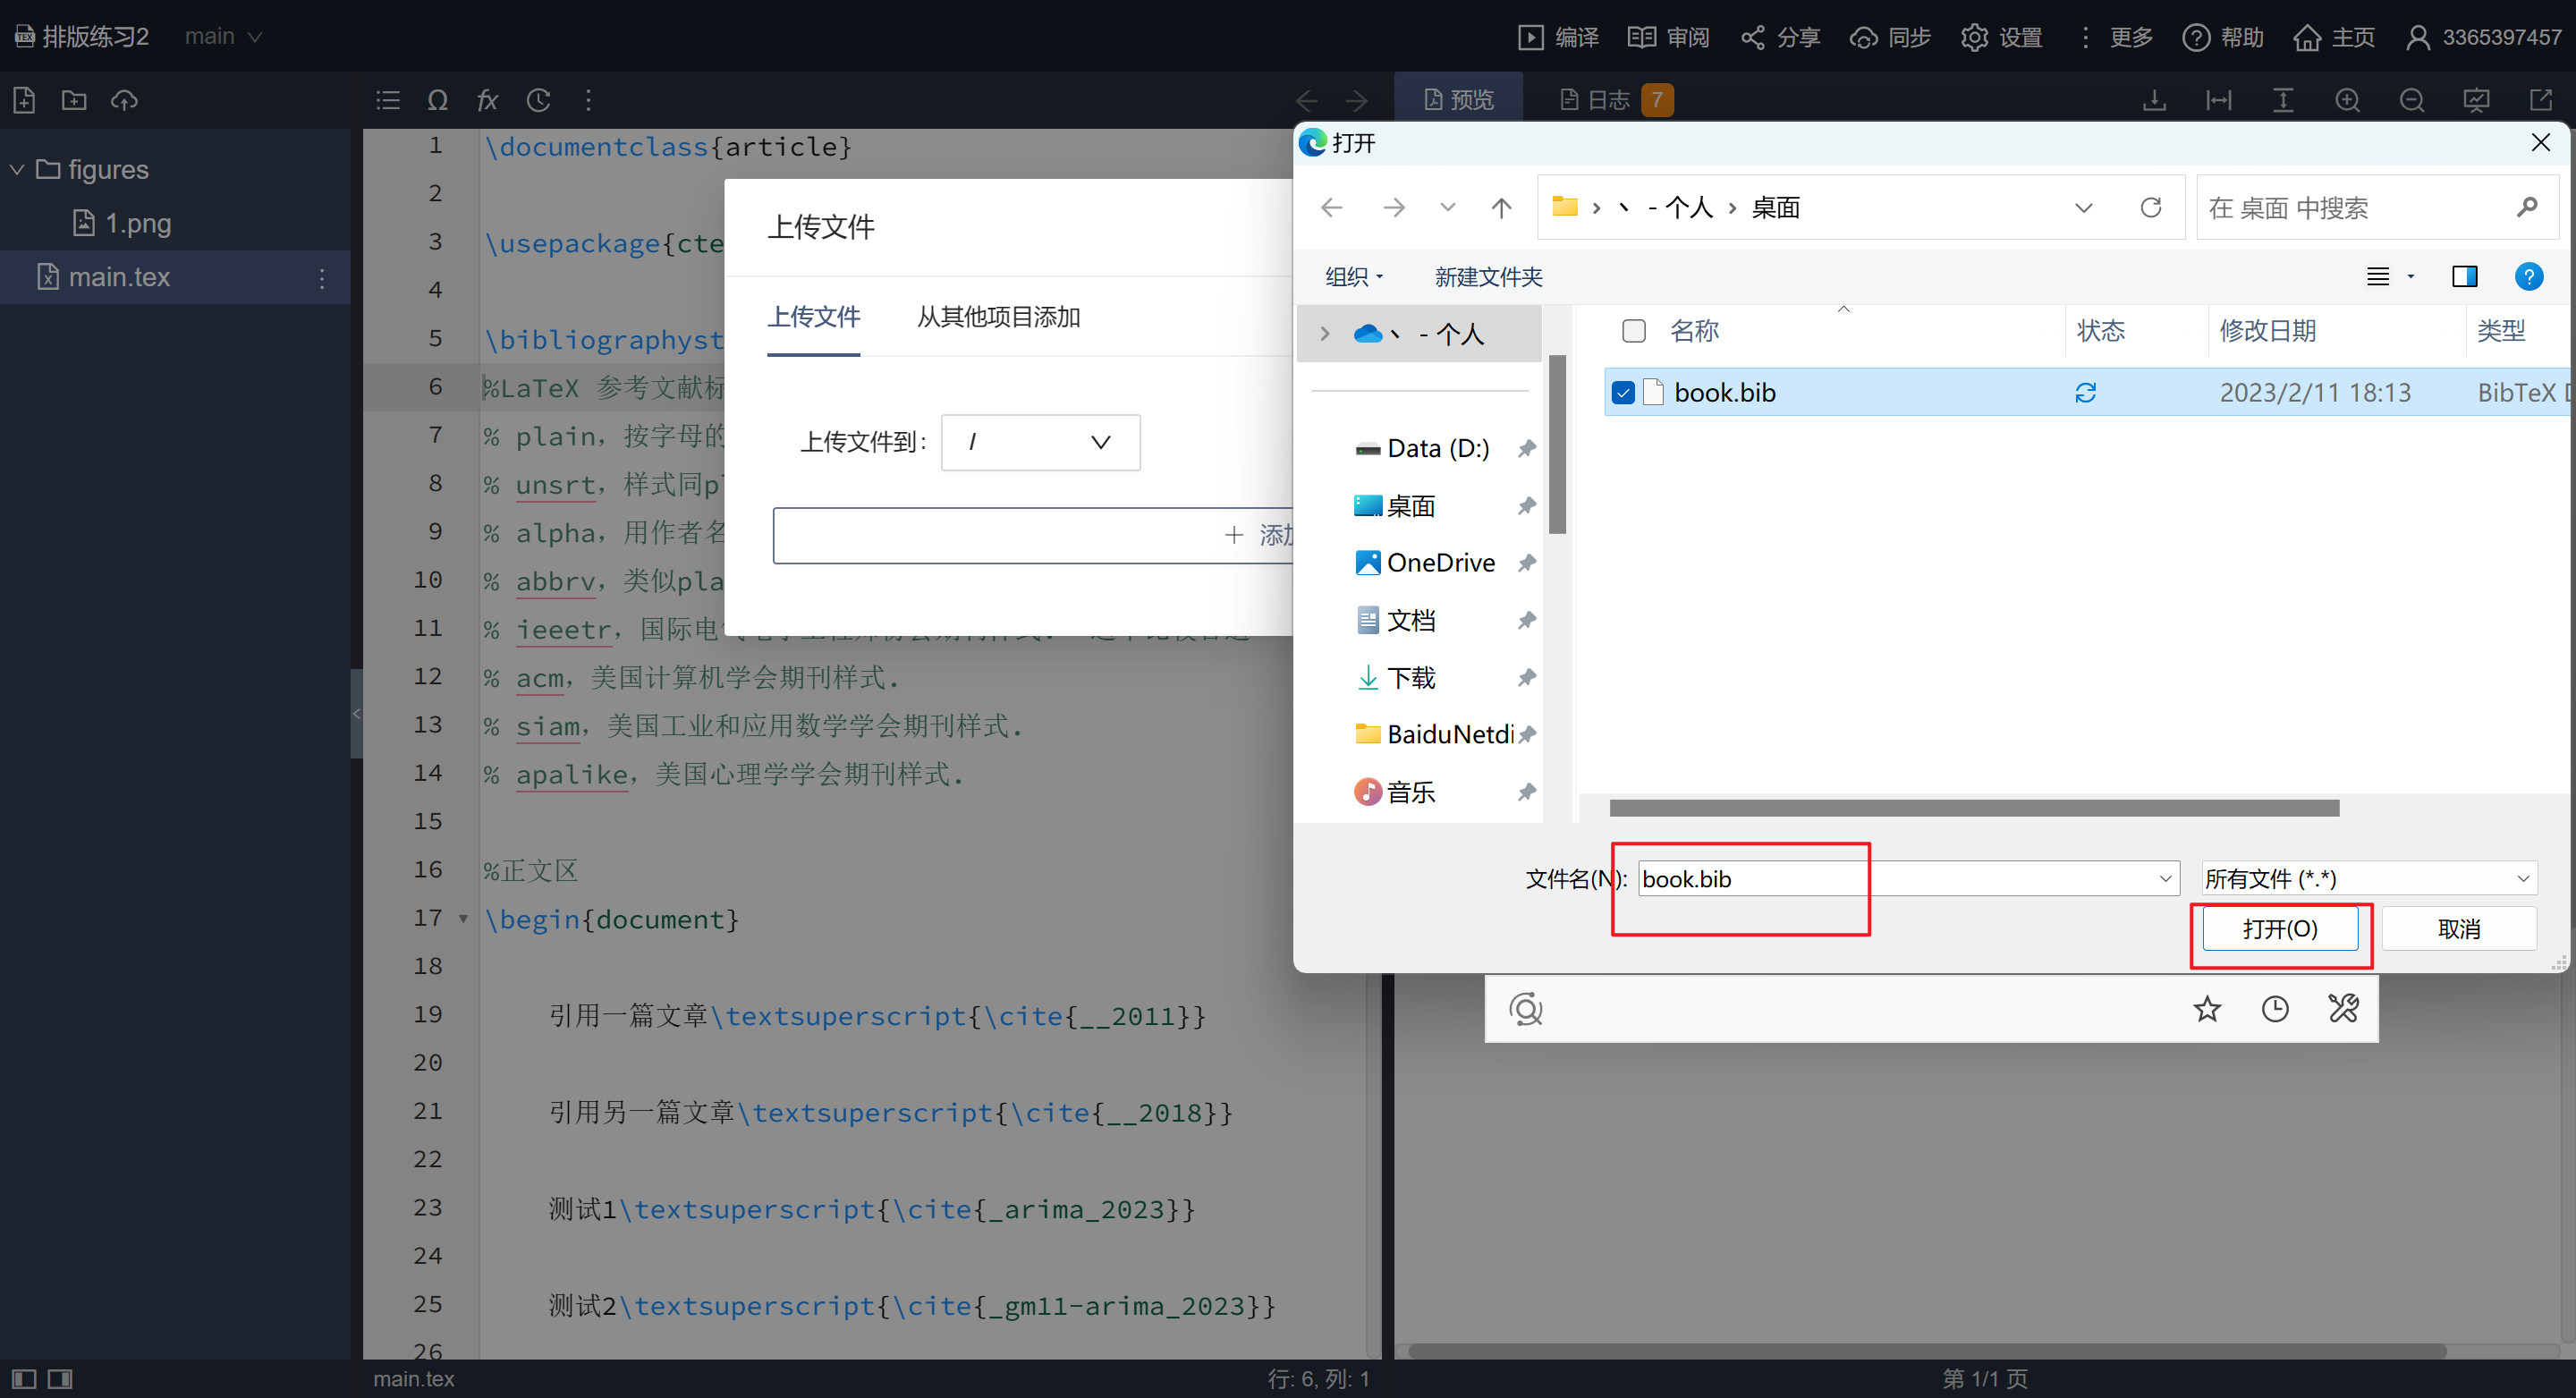
\includegraphics[width=16cm]{figure/14.png}
\end{figure}%结束引用图片环境

@article{}所选的内容就是标签,可以修改自己想要的标签
还有其他的信息都可以进行修改
\begin{figure}[H]%开始引用图片环境,[h]为固定图片,防止图片乱跑
    \centering%使图片居中
    %插入图片的命令,[scale]为图片大小,后面跟着图片的路径和名字。也可以使用width和height更改图片的大小
    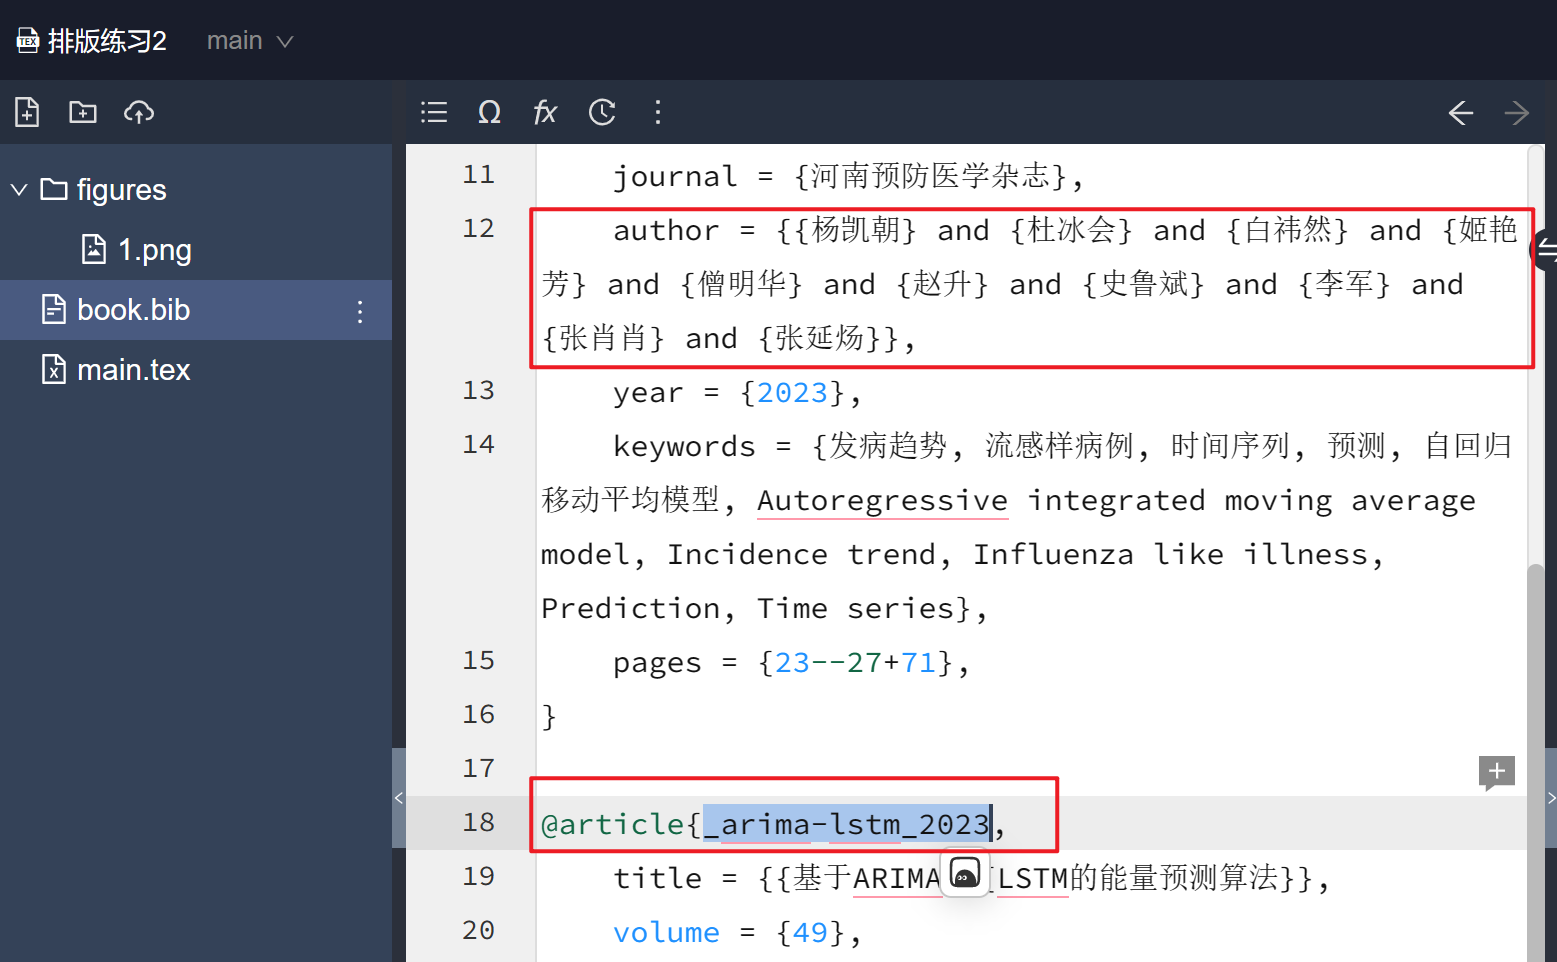
\includegraphics[width=16cm]{figure/15.png}
\end{figure}%结束引用图片环境

\begin{lstlisting}
\bibliographystyle{unsrt} %导入的参考文献风格
%LaTeX 参考文献标准选项及其样式共有以下8种:
% plain,按字母的顺序排列,比较次序为作者、年度和标题.
% unsrt,样式同plain,只是按照引用的先后排序.
% alpha,用作者名首字母+年份后两位作标号,以字母顺序排序.
% abbrv,类似plain,将月份全拼改为缩写,更显紧凑.
% ieeetr,国际电气电子工程师协会期刊样式.  这个比较合适
% acm,美国计算机学会期刊样式.
% siam,美国工业和应用数学学会期刊样式.
% apalike,美国心理学学会期刊样式.

引用一篇文章\textsuperscript{\cite{LSTM的能量预测算法}}

引用另一篇文章\textsuperscript{\cite{ARIMA组合模型}}

\bibliography{book} %bib文件名
	
\end{document}
\end{lstlisting}

引用一篇文章\textsuperscript{\cite{LSTM的能量预测算法}}

引用另一篇文章\textsuperscript{\cite{ARIMA组合模型}}

\bibliography{book} %bib文件名
	
\end{document}